% interacttfssample.tex
% v1.05 - August 2017
\documentclass[]{interact}
\usepackage[utf8]{inputenc}
\usepackage{times}
\usepackage{microtype}

\usepackage{epstopdf}% To incorporate .eps illustrations using PDFLaTeX, etc.

%\usepackage[caption=false]{subfig}% Support for small, `sub' figures and tables

%\usepackage[nolists,tablesfirst]{endfloat}% To `separate' figures and tables from text if required

%\usepackage[doublespacing]{setspace}% To produce a `double spaced' document if required
%\setlength\parindent{24pt}% To increase paragraph indentation when line spacing is doubled
%\setlength\bibindent{2em}% To increase hanging indent in bibliography when line spacing is doubled

\usepackage[numbers,sort&compress]{natbib}% Citation support using natbib.sty  %

\usepackage{subfigure}
\usepackage{multirow}
\usepackage{float}
\usepackage{soul}
\usepackage{xcolor}
\graphicspath{{./images/}}


\bibpunct[, ]{[}{]}{,}{}{,}{,}% Citation support using natbib.sty
\renewcommand\bibfont{\fontsize{10}{12}\selectfont}% Bibliography support using natbib.sty

\theoremstyle{plain}% Theorem-like structures provided by amsthm.sty
\newtheorem{theorem}{Theorem}[section]
\newtheorem{lemma}[theorem]{Lemma}
\newtheorem{corollary}[theorem]{Corollary}
\newtheorem{proposition}[theorem]{Proposition}

\theoremstyle{definition}
\newtheorem{definition}[theorem]{Definition}
\newtheorem{example}[theorem]{Example}

\theoremstyle{remark}
\newtheorem{remark}{Remark}
\newtheorem{notation}{Notation}

\begin{document}

%\articletype{ARTICLE TEMPLATE}% Specify the article type or omit as appropriate

\title{Hilbert space methods to approximate Gaussian processes using Stan}

%\author{
%\name{}
%\affil{\textsuperscript{a}Department of Cartographic Engineering, Geodesy, and Photogrammetry, Universitat Polit\`ecnica de Val\`encia, Spain; }
%}

\maketitle

\begin{abstract}

\end{abstract}

\begin{keywords}
Gaussian processes; Low-rank Gaussian processes; Hilbert Space methods; Sparse Gaussian processes
\end{keywords}

\tableofcontents


%Contents
\newpage

\section{Introduction}\label{sec:bf_intro}

Gaussian processes (GPs) are flexible statistical models for specifying probability distributions over multi-dimensional non-linear functions \citep{rasmussen2006gaussian,neal1997monte}. Their name stems from the fact that any finite set of function values is jointly distributed as a multivariate normal. GPs themselves are defined by two functions, a mean and a covariance function, with the latter being arguably the more important one. The covariance function encodes our prior assumptions about the functional relationship, such as continuity, smoothness, periodicity and scale properties. GPs not only allow for non-linear effects but can also implicitly handle interactions between covariates. Different types of covariance functions can be used, and they may be combined for further increased flexibility. Due to their generality and flexibility, GPs are of broad interest across machine learning and statistics \citep{rasmussen2006gaussian,neal1997monte}. Among others, they find application in the fields of spatial epidemiology \citep{diggle2013statistical,carlin2014hierarchical}, robotics and control \citep{deisenroth2015gaussian}, signal processing \citep{sarkka2013spatiotemporal}, as well as Bayesian optimization and probabilistic numerics \citep{roberts2010bayesian,briol2015probabilistic,hennig2015probabilistic}.

Given $n$ observations in the data, the computational comlexity and memory requirements of exact GP implementation in general scale as $O(n^3)$ and $O(n^2)$, respectively. This would limit their application to rather small data sets of a few tens of thousands observations at most. The problem becomes especially severe when performing full Bayesian inference via sampling methods, where in each sampling step we need $O(n^3)$ computations when inverting the Gram matrix of the covariance function, usually through Cholesky factorization. To alleviate these computational demands, several approximate methods have been proposed, which we will briefly review in the following. 

Sparse GPs are based on low-rank approximations of the covariance matrix. The low-rank approximation with $m \ll n$ {\it inducing points} implies reduced memory requirements of $O(nm)$ and corresponding computational complexity of $O(nm^2)$.
A unifying view on sparse GPs based on approximate generative methods
is provided in \cite{quinonero2005unifying}, while a general review
can be found in \cite{rasmussen2006gaussian}.
% More recent developments in the context of sparse GPs include a structured kernel interpolation method \citep{wilson2015kernel}. More recently, \citep{bui2017unifying} proposed to use inducing points-based sparse approximation methods to perform GP approximations at inference time rather than at modeling time.

An alternative class of low-rank approximations is based on forming a basis function approximation with $m \ll n$ basis functions. The basis functions are usually presented explicitly, but can also be used to form a low rank covariance matrix approximation. Common basis function approximations rest on the spectral analysis and series expansions of Gaussian processes \citep{loeve1977probability,trees1968detection,adler1981geometry,cramer2013stationary}.
Sparse spectrum GPs are based on a sparse approximation to the frequency domain representation of a GP \citep{lazaro2010sparse,quia2010sparse,gal2015improving}. Recently, \cite{hensman2017variational} presented a variational Fourier feature approximation for Gaussian processes that was derived for the Mat{\'e}rn class of kernels. Another related method for approximating kernels relies on random fourier features \citep{rahimi2008random,rahimi2009weighted}.
Further, certain spline smoothing basis functions are equivalent to GPs with certain covariance functions \citep{wahba1990spline}, but not all spline models are GPs (e.g., sometimes splines are not marginalization consistent).

\textcolor{red}{Paul: Can we clarify how our discussed method relates to the former paragraph,
which introduces all sorts of basis function approximations. I.e. is our method
just one out of many or what makes it special? Perhaps we can somehow use the information provided
in: While Sparse Spectrum GP is based on a sparse spectrum, the reduced-rank method proposed in this paper aims to make the spectrum as ‘full’ as possible at a given rank. Recent Splines models can reproduce the Matern family of covariance functions (see, e.g., \cite{wood2003thin}), however our approach can reproduce basically all of the stationary covariance functions.}

In this paper we focus on the basis function approximation via Laplace eigenfunctions for stationary covariance functions proposed by \citet{solin2018hilbert}. Basis function approaches behave computationally like linear models, which is an attractive property in modular probabilistic programming models where there is a big benefit id approximation specific computation is simple (Paul: What do you mean with the the last part of the sentence?). The Laplace eigenfunctions can be computed analytically and they are independent of the particular choice of the covariance kernel including the hyperparameters. While the pre-computation cost of the basis functions is $O(m^2n)$, the computational cost when only changing the covariance function parameters is $O(mn+m)$ (or even $O(m^3)$ if marginalization can be used). This is a big advantage in terms of speed for iterative algorithms such as Markov chain Monte Carlo (MCMC). Another advantage is the reduced memory requirements of automatic differentation methods used in modern probabilistic programming frameworks (cite!). This is because the memory requirements of automatic differentation rather scale with the computational complexity instead of with the usual memory requirements for the posterior density computation. The discussed basis function approach also provides an easy way to apply the non-centered parameterization of GPs, which reduces the posterior dependency between parameters representing the estimated function and the hyperparameters of the covariance function, which helps to further improve MCMC efficiency.

While \citet{solin2018hilbert} have fully developed the mathematical theory behind this specific approximation of GPs, further work is needed for its practical implementation in probabilistic programming frameworks such as Stan \citep{carpenter2017stan}. In this paper, we analyze in detail the performance and accuracy of the method in relation to key factors such as the number of basis functions, desired prediction space, or properties of the true functional relationship between covariates and response variable. We provide intuitive visualizations and practical recommendations for the choice of these factors, which will help users to improve computational performance while maintaining close approximation to exact GPs. 

Although there are several GP specific software packages available to date (GPML, GPstuff, GPy, GPflow, cite them!), each provide efficient implementations only for a restricted range of GP based models. In this paper, we do not focus on the fastest possible inference for some specific GP models, but instead are interested in how GPs can be easily used as modular components in probabilistic programming frameworks. 

The remainder of the paper is structured as follows. In Section 2, we introduce GPs and their reduced rank approximations proposed by \cite{solin2018hilbert}. In Section 3, we analyze the accuracy of these approximations under several conditions using analytical and numerical methods. Several case studies in which we fit
exact and approximate GPs to real and simulated data are provided in Section 4. We end with a discussion in Section 5.


\vspace{3mm}
\section{Method}\label{sec:bf_method}

\subsection{Gaussian process regression}

A Gaussian process (GP) is a stochastic process which defines the distribution over a collection of random variables indexed by a continuous variable, i.e. $\left\lbrace f(t): t \in \mathcal{T}\right\rbrace$ for some index set $\mathcal{T}$. Gaussian processes have the defining property that the marginal distribution of any finite subset of random variables, $\left\lbrace f(t_1), f(t_2), \hdots, f(t_K) \right\rbrace$, is a multivariate Gaussian distribution.\\

In this work, Gaussian processes will take the role of a prior distribution over function spaces for non-parametric regression in a Bayesian setting. 
Consider a data set $\mathcal{D} = \left\lbrace \mathbf{x}_n, y_n \right\rbrace_{n=1}^N$, where $y_n$ is a noisy observation of an unknown function $f$ at $\mathbf{x}_n \in \mathbb{R}^D$ , i.e. $y_n = f(\mathbf{x}_n) + \epsilon_n$. Our goal is to predict the value of the function $f^*=f(\mathbf{x}^*)$ evaluated at a new input point $\mathbf{x}^* \in \mathbb{R}^D$. That is, we want to obtain the predictive distribution $p(f^*|\mathcal{D})$ of $f^*$ conditioned on the data $\mathcal{D}$.\\

We assume a Gaussian process prior for $f \sim \mathcal{GP}(\mu(\mathbf{x}), k(\mathbf{x}, \mathbf{x}'))$, where $\mu: \mathbb{R}^D \rightarrow \mathbb{R}$ and $k: \mathbb{R}^D \times \mathbb{R}^D \rightarrow \mathbb{R}$ are the mean and covariance functions, respectively,
%
\begin{align*}
 	\mu(\mathbf{x}) &= \mathbb{E}\!\left[f(\mathbf{x})\right],\\ 
 	k(\mathbf{x}, \mathbf{x}') &= \mathbb{E}\!\left[\left( f(\mathbf{x}) - \mu(\mathbf{x}) \right)\left( f(\mathbf{x}') - \mu(\mathbf{x}') \right)\right].
\end{align*} 

The mean and covariance functions completely characterize the Gaussian process prior, and control the a priori behavior of the function $f$. Let $\mathbf{f}=\left\lbrace f(\mathbf{x}_n) \right\rbrace_{n=1}^N$, then the resulting prior distribution for $\mathbf{f}$ is a multivariate Gaussian distribution
%
\begin{align*}
\mathbf{f} \sim \mathcal{N}(\boldsymbol{\mu}, \mathbf{K}),
\end{align*}

\noindent where $\boldsymbol{\mu} = \left\lbrace \mu(\mathbf{x}_n) \right\rbrace_{n=1}^N$ is the mean and $\mathbf{K}$ the covariance matrix, where $K_{i,j}=k(\mathbf{x}_i,\mathbf{x}_j)$. The covariance function $k(\textbf{x}, \textbf{x}')$ might depend on a set of hyperparameters, $\bm{\theta}$, but we will not write this dependency explicitly to ease the notation.
The joint distribution of $\mathbf{f}$ and $f^*$ is also a multivariate Gaussian as,
%
\begin{align*}
p(\mathbf{f}, f^*)=\mathcal{N} \left( \left[ \begin{array}{cc}
\mathbf{f} \\ 
f^*
\end{array} \right] \,\middle|\, \mathbf{0},\left[ \begin{array}{cc}
\mathbf{K}_{\mathbf{f},\mathbf{f}} & \mathbf{k}_{\mathbf{f},f^*} \\ 
\mathbf{k}_{f^*,\mathbf{f}} & k_{f^*,f^*}
\end{array} \right] \right),
\end{align*} 

\noindent where $\mathbf{k}_{\mathbf{f},f^*}$ is the covariance between $\mathbf{f}$ and $f^*$, and $k_{f^*,f^*}$ is the prior variance of $f^*$. %By using the conditioning properties of multivariate Gaussian distributions, we can derive the predictive distribution for $f^*$  given $\mathbf{f}$ analytically,
% \begin{align*}
	% p(f^*| \mathbf{f}) = \mathcal{N}(f^*| \mathbf{k}_{f^*,\mathbf{f}} \mathbf{K}_{\mathbf{f},\mathbf{f}}^{-1} \mathbf{f},  k_{f^*,f^*}-\mathbf{k}_{f^*,\mathbf{f}} \mathbf{K}_{\mathbf{f},\mathbf{f}}^{-1} \mathbf{k}_{\mathbf{f},f^*}  )
% \end{align*}

{\color{red} Aki: the following until ``While Gaussian'' seems too basic to be in the paper:}

The joint distribution of the observations $\mathbf{y} = \left\lbrace y_n \right\rbrace_{n=1}^N$ and function values $\mathbf{f}$ and $f^*$, $p(\mathbf{y}, \mathbf{f}, f^*)$, is the product of the conditional distribution for $\mathbf{y}$ given $\mathbf{f}$ and the joint distribution for $\mathbf{f}$ and $f^*$,
\begin{align*}
	p(\mathbf{y}, \mathbf{f}, f^*) = p(\mathbf{y}|\mathbf{f})p(\mathbf{f}, f^*)
\end{align*}
 
By marginalizing over $\mathbf{f}$ and conditioning on vector of observations $\mathbf{y}$, we obtain the posterior distribution of interest
%
\begin{align}\label{eq:posterior}
	p(f^*|\mathbf{y}) = \frac{\int p(\mathbf{y}|\mathbf{f})p(\mathbf{f}, f^*)\text{d}\mathbf{f}}{p(\mathbf{y})},
\end{align}
where $p(\mathbf{y})$ is the marginal likelihood and is given by
\begin{align}\label{eq:evidence}
	p(\textbf{y}) = \int p(\mathbf{y}|\mathbf{f})p(\mathbf{f}, f^*) \text{d}\bm{f}\text{d}f^*.
\end{align}
%
If the observation model $p(\mathbf{y}|\mathbf{f})$ is Gaussian, both integrals in eq. \eqref{eq:posterior} and \eqref{eq:evidence} can be solved analytically conditioned on the hyperparameters. For example, an isotropic Gaussian likelihood yields the following closed-form solution
\begin{align*}
	p(f^*| \mathbf{y}) = \mathcal{N}(f^*| \textbf{k}_{f^*,\mathbf{f}} (\textbf{K}_{\mathbf{f},\mathbf{f}} + \sigma^2 \mathbf{I})^{-1} \mathbf{f},  k_{f^*,f^*}-\mathbf{k}_{f^*,\mathbf{f}} (\mathbf{K}_{\mathbf{f},\mathbf{f}} + \sigma^2 \mathbf{I})^{-1} \mathbf{k}_{\mathbf{f},f^*}  ),
\end{align*}
where $\sigma^2$ is the noise variance.

While Gaussian processes provide an elegant framework for Bayesian non-parametric regression, there are two problems that often arise in practice. 
in many modelling problems, the observation model is non-Gaussian (e.g. Binomial or Poisson regression) and therefore, the posterior distribution $p(f^*| \mathbf{y})$ is analytically intractable and cannot be obtained in closed-form. Furthermore, it is often of interest to impose a prior distribution on one or more hyperparameters and then marginalize over the uncertainty. This renders the posterior distribution intractable even in the case of a Gaussian likelihood. Approximate inference have to be used to tackle the intractable inference problem, typically based on sampling methods such as Markov chain Monte Carlo (MCMC) \citep{brooks_2011} or distributional approximations such as Laplace approximation (\citep{williams1998bayesian,rasmussen2006gaussian}, expectation propagation \citep{minka2001expectation}, or variational Bayes methods \citep{gibbs2000variational,csato2000efficient}. Secondly, due to the matrix inverse in eq.~\eqref{eq:posterior} a direct implementation of Gaussian processes scales cubicly in the number of data points, $\mathcal{O}\left(N^3\right)$,  which can be prohibitively slow for many problems of interest. 
\\
\\
In the following section, we propose an approximate framework for fast and accurate inference for Gaussian processes. Using a basis function expansion, we approximate the Gaussian process with a linear model. This representation has three main advantages: 1) it makes inference considerably faster due to the linear structure, 2) it is simple to implement, which makes it easy to use Gaussian processes as building blocks in more complicated models and can be used as latent function in non-Gaussian observational models allowing modelling flexibility, 3) it can be made arbitrary accurate and the trade-off between computational complexity and approximation accuracy can easily be controlled.
\\
\\
The covariance function is the crucial ingredient in a Gaussian process as it encodes our prior assumptions about the function, and defines a correlation structure which characterize the correlations between function values at different inputs. A stationary covariance function is a function of $\mathbf{x}-\mathbf{x}'$, such that it can be written $k(\mathbf{x},\mathbf{x}') = k(|\mathbf{x}-\mathbf{x}'|)$, which means that the covariance is invariant to translations. Isotropic covariance functions are those that are function of the distance between observations, $k(\mathbf{x},\mathbf{x}') = k(||\mathbf{x}-\mathbf{x}'||) = k(\mathbf{r})$, which means that the covariance is both translation and rotation invariant. The Mat\'ern family with half-integers is the class of isotropic covariance functions probably most commonly used, which, in the unidimensional case (i.e. $\mathbf{x}=x\in \mathbb{R}$, so $\mathbf{r}=r\in \mathbb{R}$), are
%
\begin{align}
k_{\nu=\infty}(r)&=\sigma^2 \exp(-\frac{1}{2} r^2/\ell^2), \nonumber \\
k_{\nu=\frac{1}{2}}(r)&=\sigma^2 \exp(-r/\ell), \nonumber \\
k_{\nu=\frac{3}{2}}(r)&=\sigma^2(1+\sqrt{3}r/\ell) \exp(-\sqrt{3}r/\ell), \nonumber \\
k_{\nu=\frac{5}{2}}(r)&=\sigma^2(1+\sqrt{5}r/\ell+\frac{5}{3}r^2/\ell^2) \exp(-\sqrt{5}r/\ell), \nonumber 
\end{align}

\noindent where $\nu$ is the order the kernel, and the $\ell$ and $\sigma$ are the length-scale and magnitude, respectively, of the kernel. The particular case where $\nu=\infty$ is commonly known as squared exponential (exponentiated quadratic) covariance function, and that with $\nu=1/2$ as exponential covariance function. These covariance functions can be easily generalized to the multidimensional case, with multidimensional inputs $\mathbf{x}\in \mathbb{R}^D$ and multidimensional length-scale $\boldsymbol{\ell}\in \mathbb{R}^D$ (Gabi: We should derive the multidimensional form of the previous kernels, but I have now doubts how is the multidimensional form for the Matern kernels with $\nu$=1/2, $\nu$=3/2 and $\nu$=5/2). Using a multidimensional length-scale basically turns the isotropic covariance function into non-isotropic. 

Stationary covariance functions can be represented in terms of their spectral densities \citep{rasmussen2006gaussian}. In this sense, the covariance function of a stationary process can be represented as the Fourier transform of a positive finite measure (\textit{Bochner's theorem}, see, e.g. \cite{akhiezer1993theory}). If this measure has a density, it is known as the spectral density of the covariance function, and the covariance function and the spectral density are Fourier duals, known as the \textit{Wiener-Khintchine theorem} \citep{rasmussen2006gaussian}. The spectral density functions associated with the Mat\'ern covariance functions written above are
%
\begin{align}
S_{\nu=\infty}(w)&= \sigma^2 \sqrt{2\pi} \cdot \ell \cdot \exp\left(-0.5 \ell^2 w^2\right), \\
S_{\nu=\frac{1}{2}}(w)&= 2\sigma^2 \frac{1}{\ell}\left(\frac{1}{\ell^2} + \omega^2\right)^{-1}, \\
S_{\nu=\frac{3}{2}}(w)&= 4\sigma^2 \frac{\sqrt{3}}{\ell}^{3}\left(\frac{3}{\ell^2} + \omega^2\right)^{-2}, \\
S_{\nu=\frac{5}{2}}(w)&= \frac{16}{3}\sigma^2 \frac{\sqrt{3}}{\ell}^{5}\left(\frac{5}{\ell^2} + \omega^2\right)^{-3},  
\end{align}

\noindent where variable $w$ is in the frequency domain. The $D$-dimensional spectral density functions associated with the Mat\'ern covariance functions considered in the previous section are
%
\begin{align}
S^{\ast}_{\nu=\infty}(\mathbf{w})&= \sigma^2 \sqrt{2\pi}^D \prod_{d=1}^D l_d \cdot \exp\left(-0.5 \sum_{d=1}^D l_d^2 \mathbf{w}_d^2\right), \nonumber \\
%
S^{\ast}_{\nu}(\mathbf{w})&= \frac{2^D\pi^{D/2}\Gamma(\nu+D/2)(2\nu)^{\nu}}{\Gamma(\nu)l^{2\nu}}\left(\frac{2\nu}{l^2}+4\pi^2\mathbf{w}^2 \right)^{(\nu+D/2)}, \nonumber
\end{align}

\noindent where the $D$-vector $\mathbf{w}$ is in the frequency domain.

\subsection{Hilbert space approximate Gaussian process model}

The approximate Gaussian process method, developed by \cite{solin2018hilbert} and implemented in this paper, is based on considering the covariance operator of a homogeneous (stationary) covariance function as a pseudo-differential operator constructed as a series of Laplace operators. Then, the pseudo-differential operator is approximated with Hilbert space methods on a compact subset $\Omega \subset {\rm I\!R}^D$ subject to some boundary condition. For brevity, we will refer to these approximate Gaussian processes as HSGPs (Paul: introducing such an abbreviation perhaps shortens what we are going to write in the next sections). Below, we will present the main results around HSGPs relevant for practical application. More details and mathematical proofs are provided in \cite{solin2018hilbert}.

We begin by focusing on the case of a unidimensional input space (i.e., on GPs with just a single covariate) such that $\Omega \in \{-L,L\} \subset {\rm I\!R}$, where $L$ is some positive real value to which we also refer as boundary condition. As $\Omega$ describes the interval in which the approximations are valid, $L$ plays a critical role in the accuracy of HSGPs. We will come back to this issue in Section 3.

Within $\Omega$, we can write any stationary covariance function with input values $\{x,x'\} \in \Omega$ as 
%
\begin{equation}\label{approxcov}
k(x,x') = \sum_{j=1}^\infty S_{\theta}(\sqrt{\lambda_j}) \phi_j(x) \phi_j(x'),
\end{equation} 

\noindent where $S_{\theta}$ is the spectral density of the stationary covariance function $k$ (see Section 2.1) and $\theta$ the set of hyperparameters of $k$ \citep{rasmussen2006gaussian}. The terms $\{\lambda_j\}_{j=1}^{\infty}$ and $\{\phi_j(x)\}_{j=1}^{\infty}$ are the sets of eigenvalues and eigenvectors, respectively, of the Laplacian operator. Namely, they satisfy the following eigenvalue problem in $\Omega$ when applying the Dirichlet boundary condition (other boundary conditions could be used as well):
%
\begin{eqnarray}\label{eigenproblem}
\begin{split}
-\nabla^2 \phi_j(x)&=&\lambda \phi_j(x), \hspace{1cm}  x \in \Omega \\ 
\phi_j(x)&=&0, \hspace{2cm} x \notin \Omega.
\end{split}
\end{eqnarray} 

\noindent The eigenvalues $\lambda_j>0$ are real and positive because the Laplacian is a positive definite Hermitian operator, and the eigenfunctions $\phi_j$ for the eigenvalues problem in Equation (\ref{eigenproblem}) are sinusoidal functions. Independently of the covariance function, they can be computed as
%
\begin{eqnarray}\label{bf&lambda}
\begin{split}
\lambda_j&=\left(\frac{j\pi}{2L}\right)^2, \\
\phi_j(x)&=\sqrt{\frac{1}{L}} \text{sin}\left(\sqrt{\lambda_j}(x+L)\right).
\end{split}
\end{eqnarray}

If we truncate the sum in (\ref{approxcov}) to the first $m$ terms, the approximate covariance function becomes
%
\begin{equation}
k(x,x') \approx \sum_{j=1}^m S_{\theta}(\sqrt{\lambda_j}) \phi_j(x) \phi_j(x') = \boldsymbol{\phi}(x)^\intercal \Delta \boldsymbol{\phi}(x'), \nonumber
\end{equation}

\noindent where $\boldsymbol{\phi}(x)=\{\phi_j(x)\}_{j=1}^{m} \in {\rm I\!R}^{m}$ is the column vector of basis functions, and $\Delta  \in {\rm I\!R}^{m\times m}$ is the diagonal matrix of the spectral densities $S_{\theta}(\sqrt{\lambda_j})$: 
%
\begin{eqnarray}
\Delta &=&  \begin{bmatrix}
    S_{\theta}(\sqrt{\lambda_1}) & & \\
    & \ddots & \nonumber \\
    & & S_{\theta}(\sqrt{\lambda_m}) \\
  \end{bmatrix}.
\end{eqnarray}

Thus, the Gram matrix $\text{K}$ of the covariance function $k$ for a set of observations $i=1,\ldots,n$ and corresponding input values $\{x_i\}_{i=1}^{n} \in \Omega^{n}$ can be represented as
%
\begin{equation}
\text{K}= \Phi \Delta \Phi^\intercal, \nonumber
\end{equation}

\noindent where $\Phi \in {\rm I\!R}^{n\times m}$ is the matrix of eigenfunctions $\phi_j(x^i)$:
%
\begin{eqnarray}
\Phi &=&  \left[ {\begin{array}{ccc}
   \phi_1(x_1) & \cdots & \phi_m(x_1)  \\
    \vdots &\ddots & \vdots  \nonumber \\ 
    \phi_1(x_n) & \cdots & \phi_m(x_n) \\
  \end{array} } \right].
\end{eqnarray}
 
\noindent As a result, the model for $f$ can be written as
%
\begin{equation}
\mathbf{f} \sim \mathcal{N}(\boldsymbol{\mu},\Phi \Delta \Phi^\intercal). \nonumber
\end{equation}

\noindent This equivalently leads to a linear representation of $f$ via
%
\begin{equation}\label{approxf}
f(x) \approx \sum_{j}^m \left( S_{\theta}(\sqrt{\lambda_j})\right)^{1/2} \phi_j(x) \beta_j,
\end{equation}

\noindent where $\beta_j \sim \text{Normal}(0,1)$. Thus, the function $f$ is approximated with a finite basis function expansion (using the eigenfunctions $\phi_j$ of the Laplace operator), scaled by the square root of spectral density values. A key property of this approximation is that the eigenfunctions $\phi_j$ do not depend on the covariance hyperparameters $\theta$. Instead, the only dependence on $\theta$ is through the spectral density $S_{\theta}$. The eigenvalues $\lambda_j$ are monotonically increasing with $j$ and $S_{\theta}$ goes rapidly to zero for bounded covariance functions. Therefore, Equation (\ref{approxf}) can be expected to be a good approximation for a finite number of $m$ terms in the series as long as the inputs values $x_i$ are not too close to the boundaries $-L$ and $L$ of $\Omega$. The computational cost of univariate HSGPs scales as $O(nm + m)$, where $n$ is the number of observations and $m$ the number of basis functions.

The parameterization in \ref{approxf} is naturally in the non-centered
parameterization form with independent prior distribution on
$\beta_j$, which makes the posterior inference easier.

\subsection{Generalization to multidimensional GPs}

The results from the previous section can be generalizes to a multidimensional input space with compact regular domain $\Omega=[-L_1,L_1] \times \dots \times [-L_d,L_d]$ and Dirichlet boundary conditions. 
In a $D$-dimensional input space, the total number of eigenfunctions and eigenvalues in the approximation is equal to the number of $D$-tuples, that is possible combinations of univariate eigenfunctions over all dimensions. The number $D$-tuples is given by $m^{\ast} = \prod_{d=1}^{D} m_d$, where $m_d$ is the number of basis function for the dimension $d$. Let $\mathbb{S}\in {\rm I\!N}^{m^{\ast} \times D}$ be the matrix of all those $D$-tuples. For example, suppose we have $D=3$ dimensions and use $m_{1}=2$, $m_{2}=2$ and $m_{3}=3$ eigenfunctions and eigenvalues for the first, second and third dimension, respectively. Then, the number of multivariate eigenfunctions and eigenvalues is $m^{\ast} = m_{1} \cdot m_{2} \cdot m_{3} = 12$ and the matrix $\mathbb{S}\in {\rm I\!N}^{12 \times 3}$ is given by
\begin{align}\small
\mathbb{S}=
\left[ {\begin{array}{ccc}
1 & 1 & 1 \nonumber \\
1 & 1 & 2 \\
1 & 1 & 3 \\
1 & 2 & 1 \\
1 & 2 & 2 \\
1 & 2 & 3 \\
2 & 1 & 1 \\
2 & 1 & 2 \\
2 & 1 & 3 \\
2 & 2 & 1 \\
2 & 2 & 2 \\
2 & 2 & 3 
\end{array} } \right]
\end{align} 

Each multivariate eigenfunction $\phi^{\ast}_j$ corresponds to the product of the univariate eigenfunctions whose indices corresponds to the elements of the $D$-tuple $\mathbb{S}_{j\cdotp}$, and each multivariate eigenvalue $\lambda^{\ast}_j$ is a $D$-vector with elements that are the univariate eigenvalues whose indices correspond to the elements of the $D$-tuple $\mathbb{S}_{j\cdotp}$. Thus, for $\mathbf{x}^D \in \Omega$ and $j=1,\ldots,m$, we have 
%
\begin{align} \label{bf&lambda_multi}
\begin{split}
\phi^{\ast}_j(\mathbf{x}) &= \prod_{d=1}^{D} \phi_{\mathbb{S}_{jd}}(x_d) = \prod_{d=1}^{D} \sqrt{\frac{1}{L_d}} \text{sin}\left(\sqrt{\lambda_{\mathbb{S}_{jd}}}(x_d+L_d)\right) \\
%
\lambda^{\ast}_j &= \left\{ \lambda_{\mathbb{S}_{jd}} \right\}_{d=1}^D =  \left\{ \left(\tfrac{\pi \mathbb{S}_{jd}}{2L_d}\right)^2 \right\}_{d=1}^D. 
\end{split}
\end{align}

\noindent The approximate covariance function is then represented as
%
\begin{equation}\label{approxcov_multi}
k(\mathbf{x},\mathbf{x}') \approx \sum_{j=1}^{m^{\ast}} 
S^{\ast}_{\theta}\left(\sqrt{\lambda^{\ast}_j}\right)
\phi^{\ast}_j(\mathbf{x}) \phi^{\ast}_j(\mathbf{x}'),
\end{equation}

\noindent where $S^{\ast}_{\theta}$ is the spectral density of the $D$-dimensional covariance function (see Section 2.1). We can now write the approximate series expansion of the multivariate function $f$ as,
%
\begin{equation}\label{approxf}
f(\mathbf{x}) \approx \sum_{j=1}^{m^{\ast}} 
\left( S^{\ast}_{\theta} \left(\sqrt{\lambda^{\ast}_j} \right)\right)^{1/2}
\phi^{\ast}_j(\mathbf{x}) \beta_j, 
\end{equation}

\noindent where, again, $\beta_j \sim \text{Normal}(0,1)$. The computational cost of multivariate HSGPs scales as $O(n m^{\ast} + m^{\ast})$, where $n$ is the number of observations and $m^{\ast}$ is the number of multivariate basis functions. Although this still implies linear scaling in $n$, the approximation is more costly than in the univariate case, as $m^{\ast}$ is the product of the number of univariate basis functions over the input dimensions and grows exponentially with respect to the number of  dimensions.

\subsection{Learning hyperparameters and model inference}

\vspace{2mm}
$\bullet$ It has an attractive computational cost as this basically turns the regular GP model into a linear model.

\vspace{2mm}
$\bullet$ The design matrix of the proposed linear model, which is composed of a basis of Laplace eigenfunctions, can be computed analytically and does not depend on the hyperparameters of the model, then it has to be computed only once with $O(n+m)$ computational demands.

\vspace{2mm}
$\bullet$ The weights associated to the basis functions in this linear model is a $m$-dimensional vector ($m$ is the number of basis functions) and their computation is an operation with $O(m)$ computational demands. The weights depend on the hyperparameters, then they have to be computed in every step of the HMC sampling method.

\vspace{2mm}
$\bullet$ The linear model is computed with complexity $O(nm)$, computed in every step of the HMC sampling method.

\vspace{2mm}
$\bullet$ In a fully Bayesian inference framework using sampling methods, the proposed approximate GP model has a computational complexity of $O(nm+m)$ in every step of the HMC method. In addition, the computation of the automatic differentiation to compute the gradients in this linear model scales $O(n)$?, an operation that must be computed in every step of the HMC method.

\vspace{2mm}
$\bullet$ Using maximizing marginal likelihood methods, the proposed model has a overall complexity of $O(nm^2)$. After this, evaluating the marginal likelihood and marginal likelihood gradients is an $O(m^3)$ operation in every step of the optimizer. (Arno's paper, pag. 7)

\vspace{2mm}
$\bullet$ The parameter posterior distribution in this approximate GP model is $m$-dimensional ($m<<n$) which helps the use of GP priors as latent functions. especially when sampling methods for inference are used. GP prior as latent functions is needed in generalized models.

In regular GPs and other approximate GP models and Splines models these features do not have so nice properties:

\vspace{2mm}
$\bullet$ In a regular GPs, the main computational complexity comes from the inversion of the covariance matrix which is in general a $O(n^3)$ operation. This operation has to be computed at every step of the HMC or optimizer.

\vspace{2mm}
$\bullet$ In regular GPs, the parameter posterior distributions is $N$-dimensional. It is known that when $N$ is of medium or large size there is high correlation between the $N$-dimensional latent function and the hyperparameters of the GP prior.

\vspace{2mm}
$\bullet$ In conventional sparse GP approximations, although the rank of the GP is reduced considerably to the number of inducing points, this still needs to do the autodiff and covariance matrix inversion.

\vspace{2mm}
$\bullet$ The Splines models are also a sort of basis functions expansion model, then the computational demands are similar to that in this approach. However in Splines models the lengthscale hyperparameter tend to be fixed and then the fit is covered by the magnitude parameter. In that sense, Splines models tend to loose the useful interpretation of the lengthscale parameter.

\vspace{2mm}
$\bullet$ In addition, the computation of the automatic differentiation to compute gradients in this linear model scales $O(n)$, which is an operation that must be computed in every step of the HMC method.

\vspace{2mm}
$\bullet$ In a regular GP model the automatic differentiation to compute the gradients of the covariance function scales $O(n^2)$, the dimension of the covariance matrix, and the full inversion of the covariance matrix scales $O(n^3)$. This operation has to be computed at every step of the HMC.

\vspace{2mm}
$\bullet$ In a sparse GP approach based on inducing points, although the rank of the GP is reduced considerably to the number of inducing points, this still needs to do the autodiff and covariance matrix inversion.

\vspace{2mm}
$\bullet$ The Splines models are also a sort of basis functions expansion model, then the computational demands are similar to that in this approach.


\section{The accuracy of the approximation}

Implementation and performance of the HSGP model depends on the number of basis functions and boundary settings, which are, at the same time, related  to each other. The time of computation in the approximation mainly depends on the number of basis functions. Furthermore, the appropriate values for the number of basis functions and boundary depend on the non-linear functional effects of the function characterized by the lengthscale of the covariance function.

In this section we analyze the effects of the number of basis functions and boundary on the approximation accuracy. We present recommendations how they should be chosen and diagnostics to check the accuracy of the approximation after the inference.
We illustrate graphically how the number of basis functions, boundary and lengthscale relate to each other and affect the accuracy of the approximation.
% This graph basically provides the recommended values for these factors in order to get a close approximation. This graph also allows us to diagnose an actual fit by checking whether the value of the estimated lengthscale does not keep to those that the Figure brings as suitable ones.

We compare regular GP and HSGP fitted for different dataset with different "wigglyness".
%The comparison is made through comparing their estimated lengthscales. 

\subsection{Dependency on the number of basis functions and the boundary condition}

The approximation of the covariance function is a series expansion of eigenfunctions and eigenvalues of the Laplace operator in a given domain $\Omega$, e.g. in a 1-$D$ input space $x\in \Omega=[-L,L]\subset \mathbb{R}$:
%
\begin{equation}\label{diffcov}
k(\tau) = \sum_{j}^{\infty} S_{\theta}(\sqrt{\lambda_j}) \phi_j(\tau) \phi_j(0),  \nonumber
\end{equation} 

\noindent where $L$ is the boundary, $j$ is the index for the eigenfunctions and eigenvalues, and $\tau=x-x'$. The eigenvalues $\lambda_j$ and eigenfunctions $\phi_j$ are those in equation (\ref{bf&lambda}) for the unidimensional case and those in equation (\ref{bf&lambda_multi}) for the multidimensional case.

The approximation to the covariance function becomes exact in the limit when the number of basis functions approach infinity, $j=1,\cdots,\infty$. The number of basis functions can be truncated at some finite positive value $m$ such that the difference between the densities of the exact and approximate covariance functions be less than a threshold $\epsilon$,
%
\begin{eqnarray}\label{diff_covs}
\int k(\tau)d(\tau) - \int \sum_{j}^m S_{\theta}(\sqrt{\lambda_j}) \phi_j(\tau) \phi_j(0) d(\tau) < \epsilon.
\end{eqnarray}

The finite number $m$ of basis functions in the approximation needed to satisfy eq. (\ref{diff_covs}) depends on the non-linear effects of the function to be learned, that is, on its lengthscale $\ell$. The approximation also depends on boundary $L$ (equations (\ref{bf&lambda}) and (\ref{bf&lambda_multi})) which will affect the performance specially near the boundaries. The boundary will also have an effect on the number of basis functions needed in the approximation. The boundary $L$ is set as an extension of the desired predicting input domain $\Psi$. Considering a zero-mean input domain $\Psi=[-S,S] \in \mathbb{R}$, the boundary is defined as
%
\begin{equation}
L=c \cdot S,
\end{equation} 

\noindent where $S$ represents the half-range of the input space, and $c$ ($c \ge 1$) is the proportional extension factor. From now on we are going to refer to this proportional factor $c$ as the boundary factor of the approximation. The boundary factor can also be regarded as the boundary $L$ normalized by the half-range $S$ of the input space.

For a naive illustration of the effects of these two factors, number of basis functions $m$ and boundary $L$, on the performance of the approximation, a set of noisy observations are drawn from a GP model with lengthscale $\ell=0.3$ and marginal variance $\alpha=1$, and input vales within the zero-mean input domain with half-range $S=1$. HSGP models with different number of basis functions and boundaries are fitted to this data. The lengthscale and marginal variance parameters are considered fixed to the true values of the data-generative GP model. Figures \ref{fig1_Post_J} and \ref{fig2_Post_L} illustrate the individual effects of the number of basis functions and the boundary, respectively, on the approximation of the covariance function. On the one hand, for a fixed $L$, let's suppose it is set to a right choice, Figure \ref{fig1_Post_J} shows the effect of changing the number of basis functions in approaching the posterior mean and the covariance function. It can be seen how the number of basis functions affects the non-linear effects of the posteriors. Fewer basis functions implies smoother covariance functions and consequently smoother posteriors. The more "wigglyness" of the function, the more basis functions are needed. On the other hand, and similarly, for a fixed number of basis functions $m$, let's suppose it is set to a right choice, Figure \ref{fig2_Post_L} shows the effect of changing the boundary $L$ in approaching the posterior mean and the covariance function. It can be seen how the box size mainly affects the approximation near the boundaries of the function and affects the covariances at long distances. \\

\begin{figure}
\centering
\subfigure{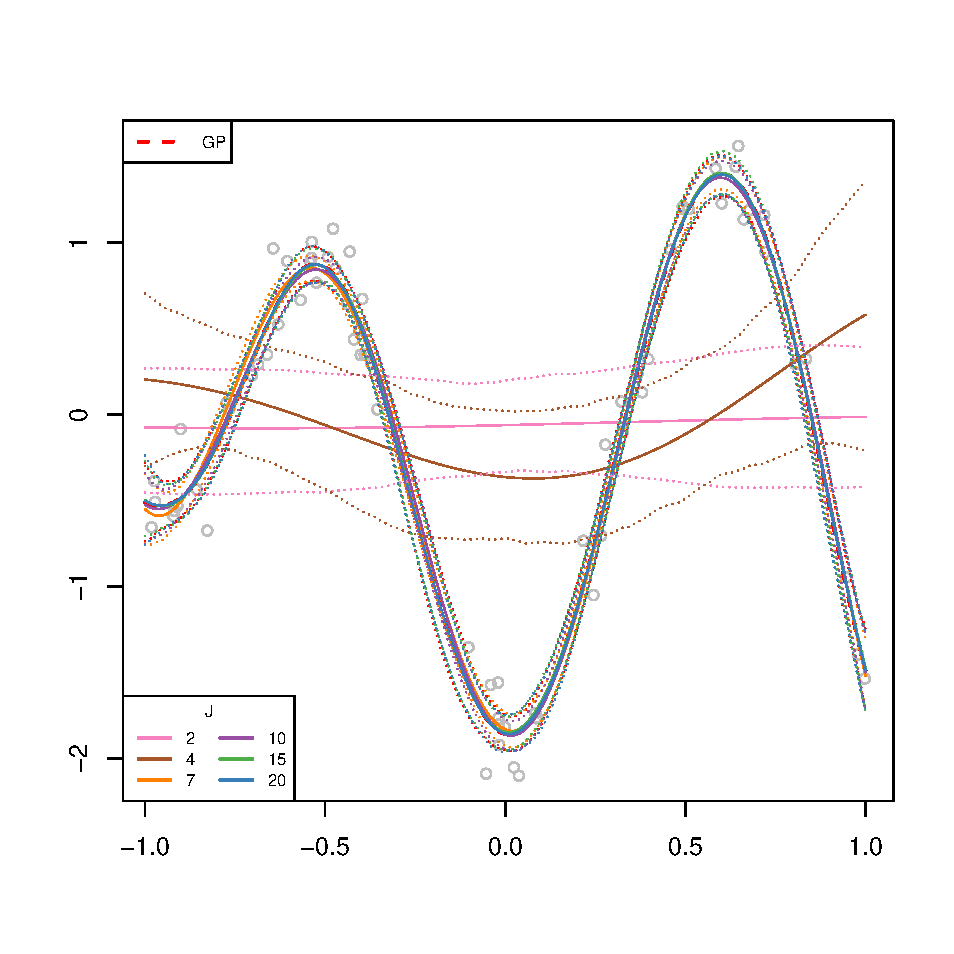
\includegraphics[scale=0.43, trim = 0mm 0mm 0mm 10mm, clip]{fig1_Post_J.pdf}}
\subfigure{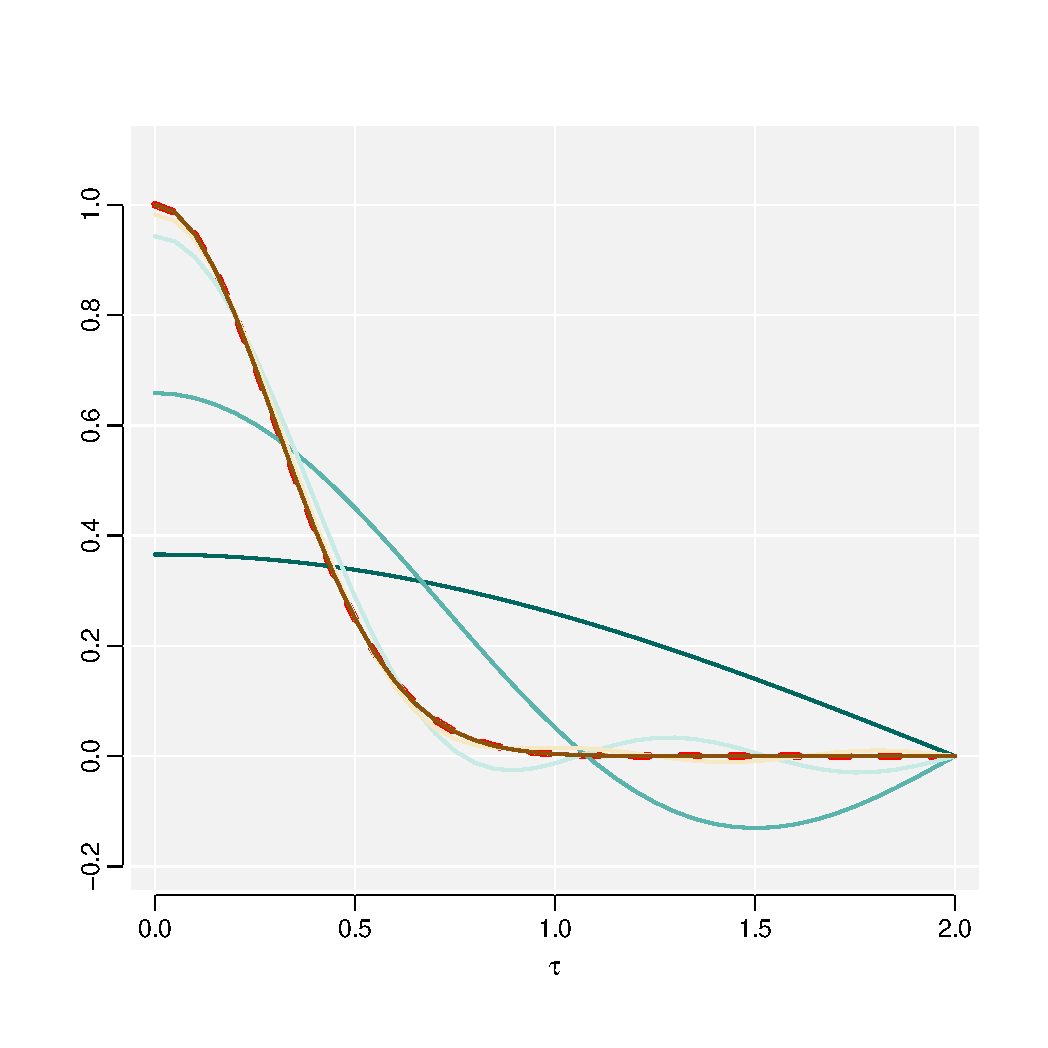
\includegraphics[scale=0.43, trim = 0mm 0mm 0mm 10mm, clip]{fig1_Cov_J.pdf}}
\caption{(left) Posterior distributions for different number of basis functions $m$. (right) Covariance function for different number of basis functions $m$.}
  \label{fig1_Post_J}
\end{figure}


\begin{figure}
\centering
\subfigure{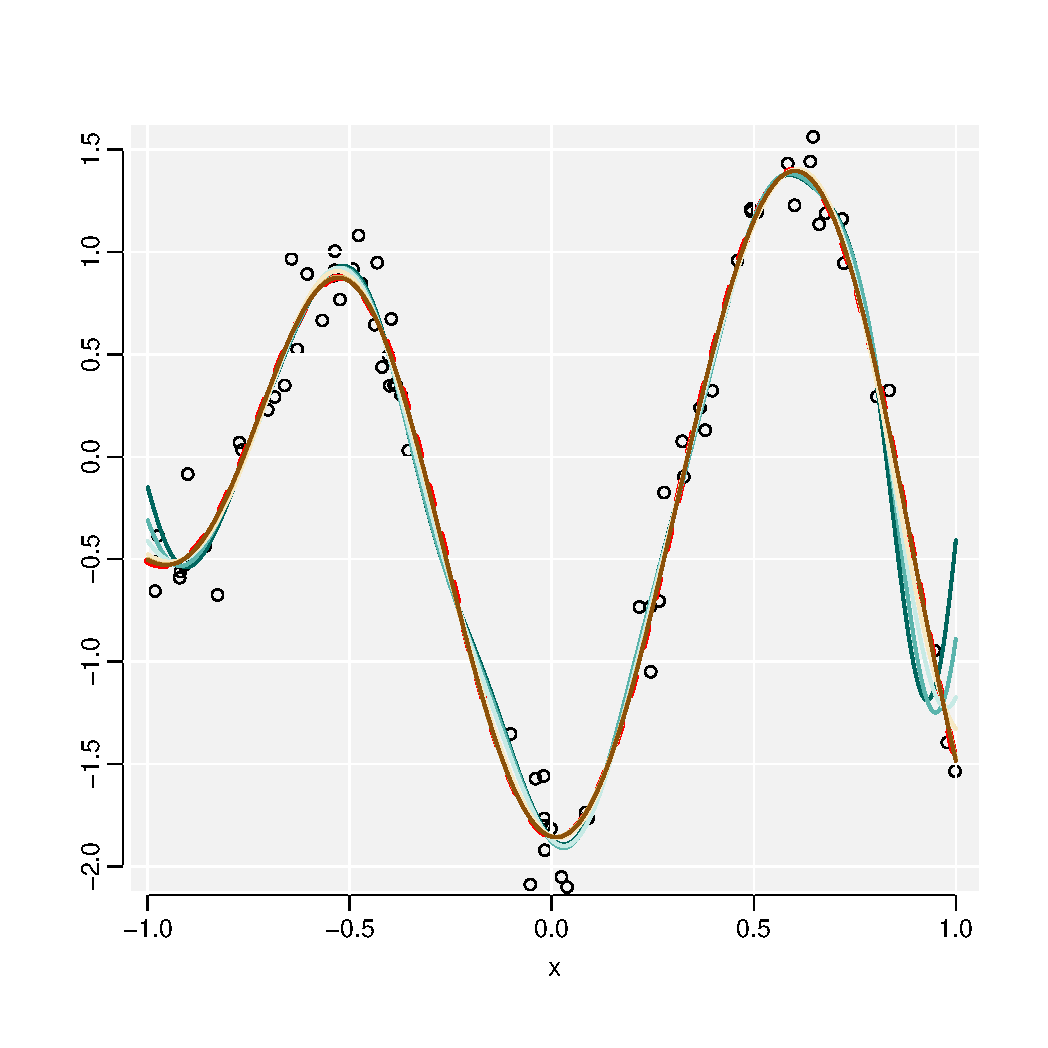
\includegraphics[scale=0.43]{fig2_Post_L.pdf}}
\subfigure{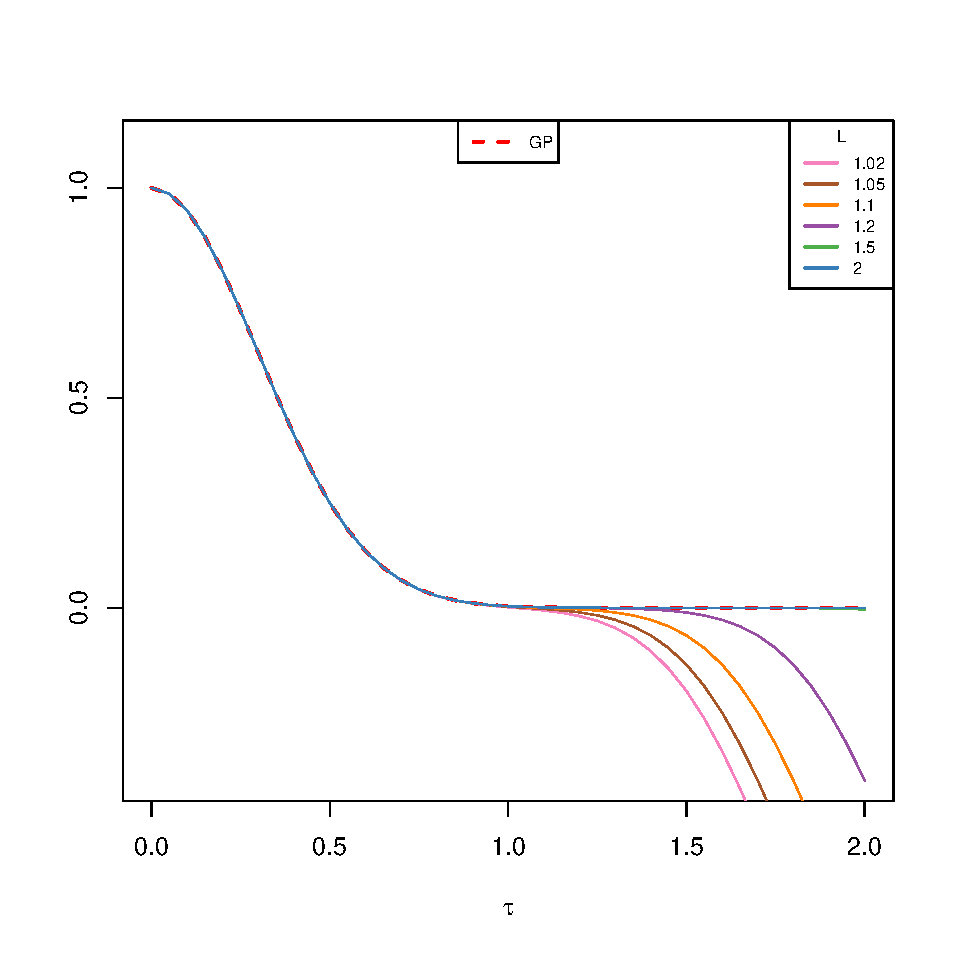
\includegraphics[scale=0.43]{fig2_Cov_L.pdf}}
\caption{(left) Posterior means for different different values of the box size $L$. (right) Covariance functions for different values of the box size $L$.}
  \label{fig2_Post_L}
\end{figure}


In the previous Figures \ref{fig1_Post_J} and \ref{fig2_Post_L} we focused on illustrating the individual effects of the number of basis functions and the boundary. Furthermore, for a clearer illustration of these effects, the lengthscale and marginal variance parameters in the HSGP model were fixed to their true values. Now we are going to focus on analyzing the interaction effects between these two factors, number of basis functions and the boundary factor, on the performance of the approximation. The lengthscale and marginal variance will not be fixed rather they will be estimated either in regular and HSGP models.  
%The right-side plots in Figures \ref{fig1_Post_J} and \ref{fig2_Post_L} are computed using the lengthscale and magnitud values of the true GP prior. Now, we focus on the estimated lengthscale and magnitud parameters after fitting the model, either of the regular GP model fit and approximate GP model fit. 
Figure \ref{fig4_Post_&_Cov_part1} shows the posteriors means and the covariance functions obtained after fitting the data, for different number of basis functions and boundary factor. Figure \ref{fig5_MSE_vs_J} shows the root mean square error (RMSE) of the approximate GP model, computed against the regular GP model, as a function of the number of basis functions and the boundary factor. Figure \ref{fig6_lscale_vs_J} shows the lengthscale and marginal variance for the regular GP model and for the HSGP models as a function of the number of basis functions and boundary factor. Looking at the RMSEs in Figure \ref{fig5_MSE_vs_J}, it can be drawn that the optimal choice in terms of precision and computations would be 15 basis functions and a boundary factor between 1.5 and 2.5. The choice of 10 basis functions and a boundary factor of 1.5 could be an accurate enough choice. This same conclusion can be also be intuitively seen in the posterior mean and covariance function plots in Figure \ref{fig4_Post_&_Cov_part1}.

From Figure \ref{fig5_MSE_vs_J}, a behaviour in terms of performance of the HSGP model as a function of the number of basis functions and the boundary factor, can be deduced: \\
$\bullet$ as the boundary factor increases, more basis functions are needed,
\\
$\bullet$ as fewer basis functions are used, the boundary factor must decrease. 

Similar conclusions can be stated from results of Figure \ref{fig6_lscale_vs_J}. This Figure shows the estimated lengthscale and marginal variance as function of the number of basis functions and boundary factor. In addition to the above conclusions, in Figure \ref{fig6_lscale_vs_J} it can be easily seen that exists a minimum value for the boundary factor under which a close approximation will never be achieved. \\

\begin{figure}
\centering
\subfigure{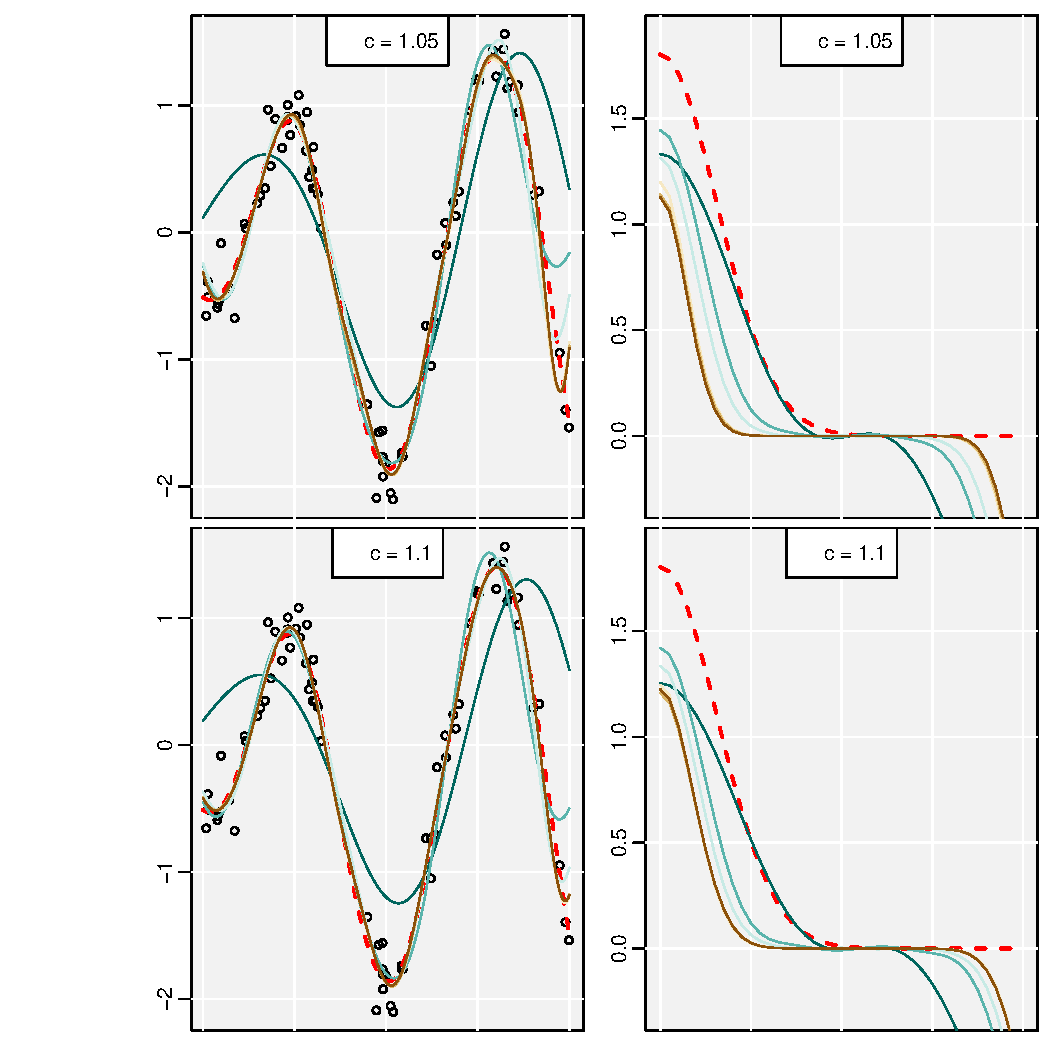
\includegraphics[scale=0.6]{fig4_Post_&_Cov_part1.pdf}}
\subfigure{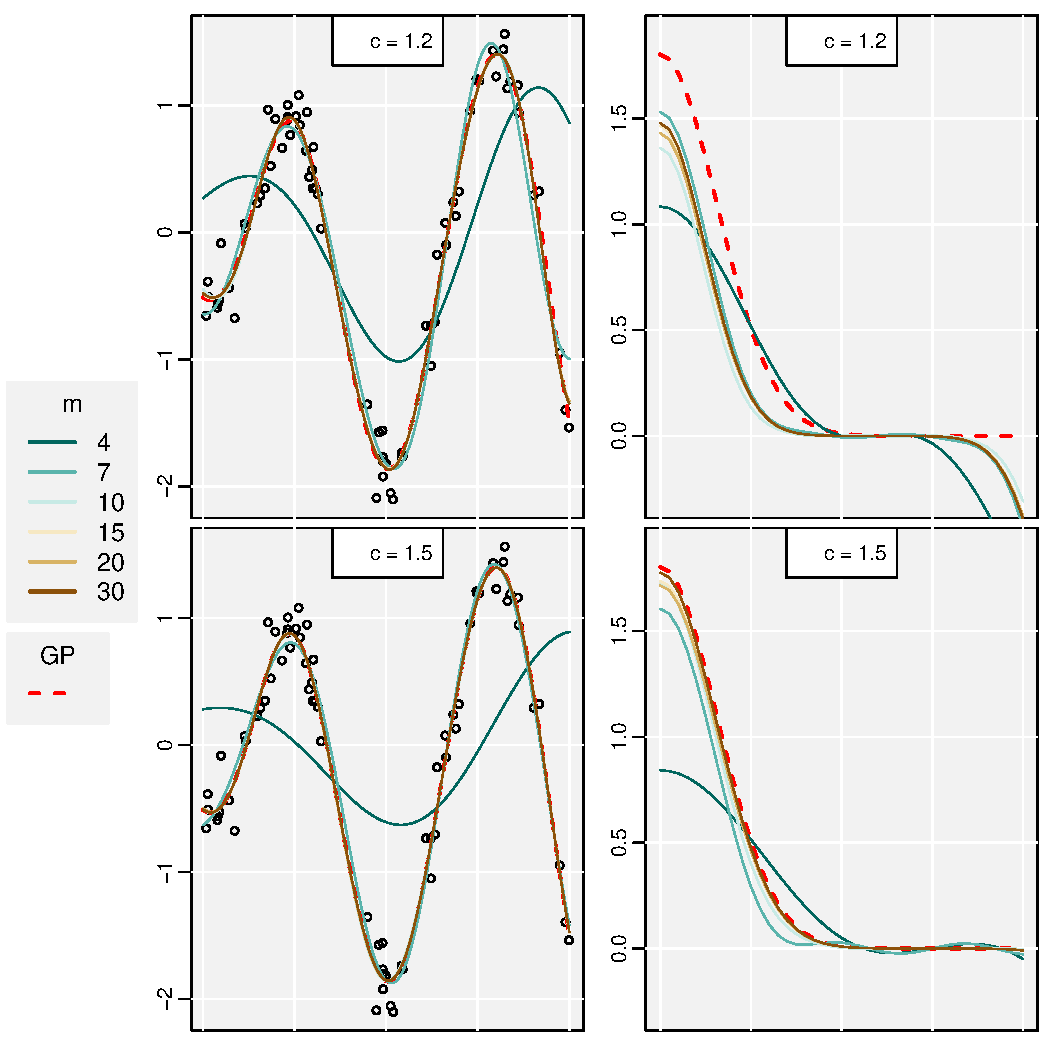
\includegraphics[scale=0.6]{fig4_Post_&_Cov_part2.pdf}}
\caption{Posterior distributions and covariance functions of the regular GP model and the proposed HSGP model as a function of the number of basis functions $m$ and the boundary factor $c$.} 
  \label{fig4_Post_&_Cov_part1}
\end{figure}

\begin{figure}
\centering
\subfigure{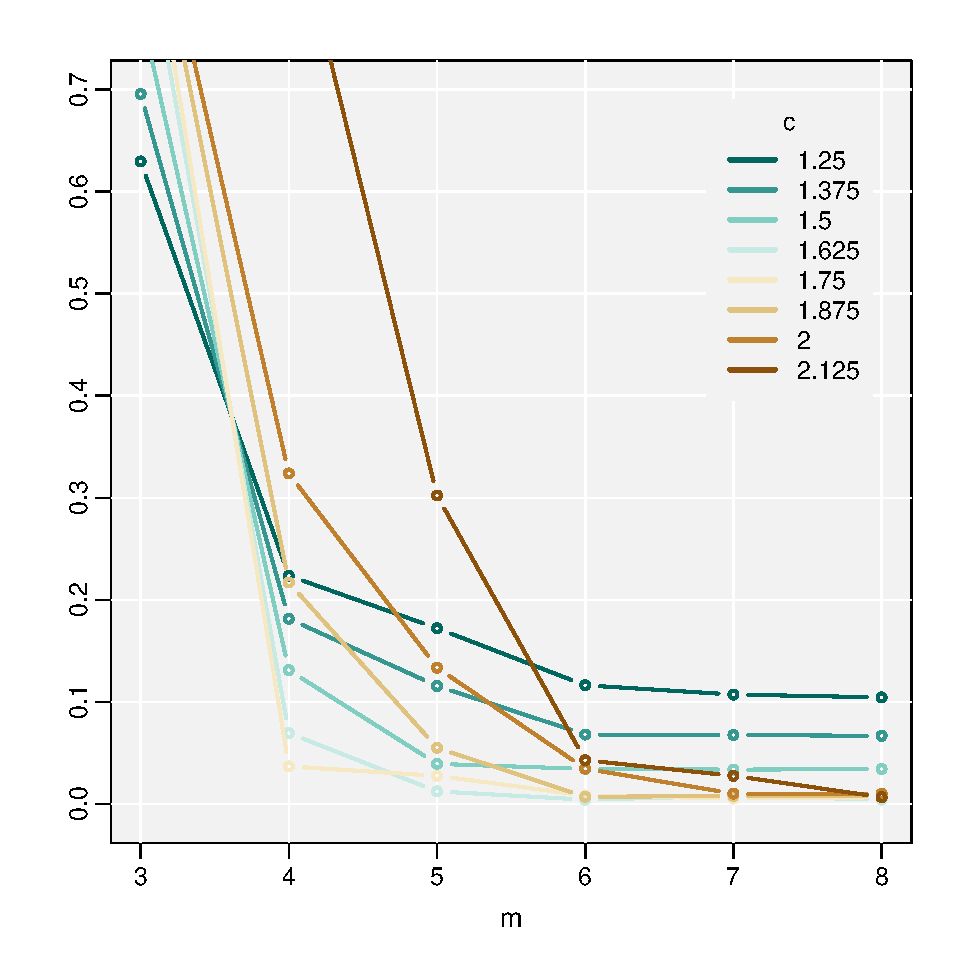
\includegraphics[scale=0.4]{fig5_MSE_vs_J.pdf}}
\subfigure{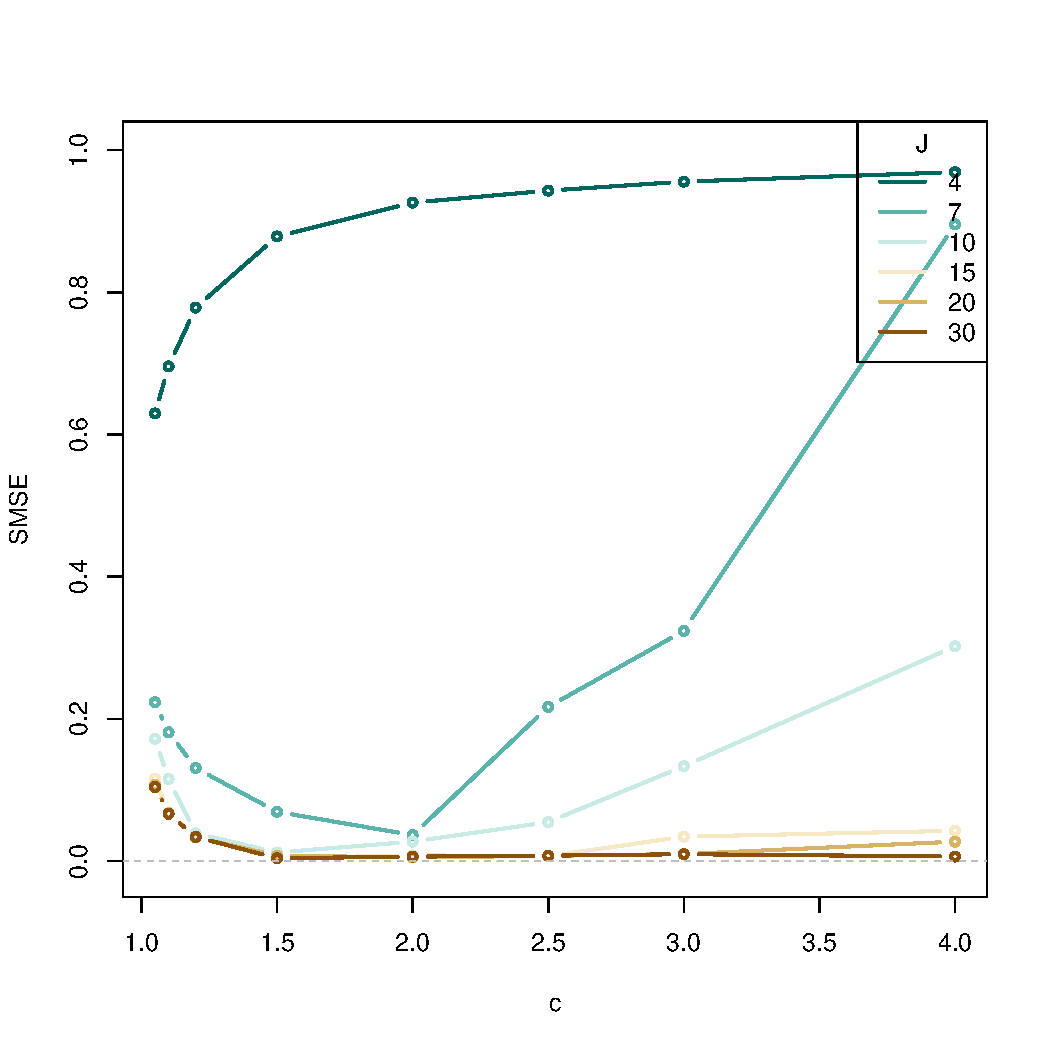
\includegraphics[scale=0.4]{fig5_MSE_vs_c.pdf}}
\caption{Standardized root mean square error (SRMSE) of the proposed HSGP models computed against the regular GP model. (left) SRMSE vs the number of basis functions $m$ and for different values of the boundary factor $c$. (right) SRMSE vs the boundary factor $c$ and for different values of the number of basis functions $m$. }
  \label{fig5_MSE_vs_J}
\end{figure}

\begin{figure}
\centering
\subfigure{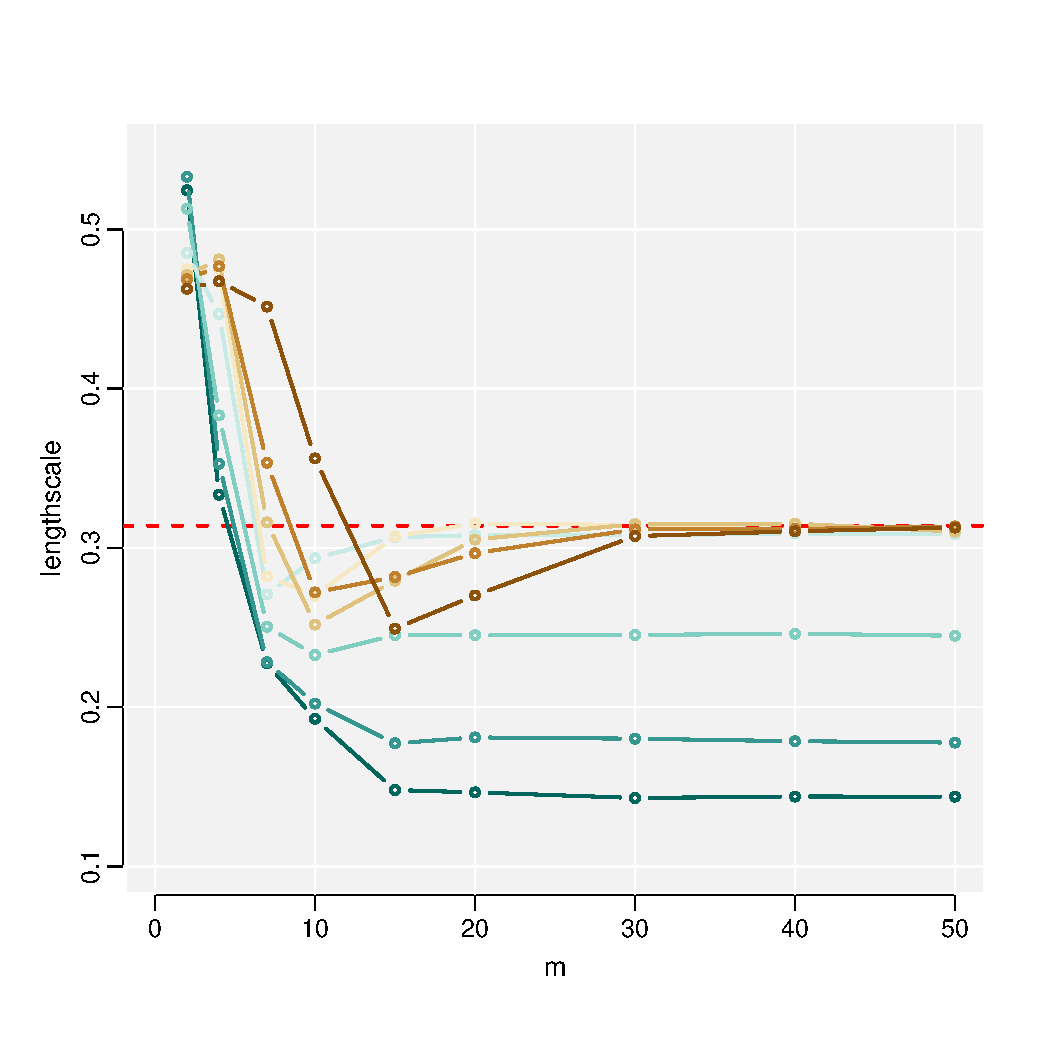
\includegraphics[scale=0.4]{fig6_lscale_vs_J.pdf}}
\subfigure{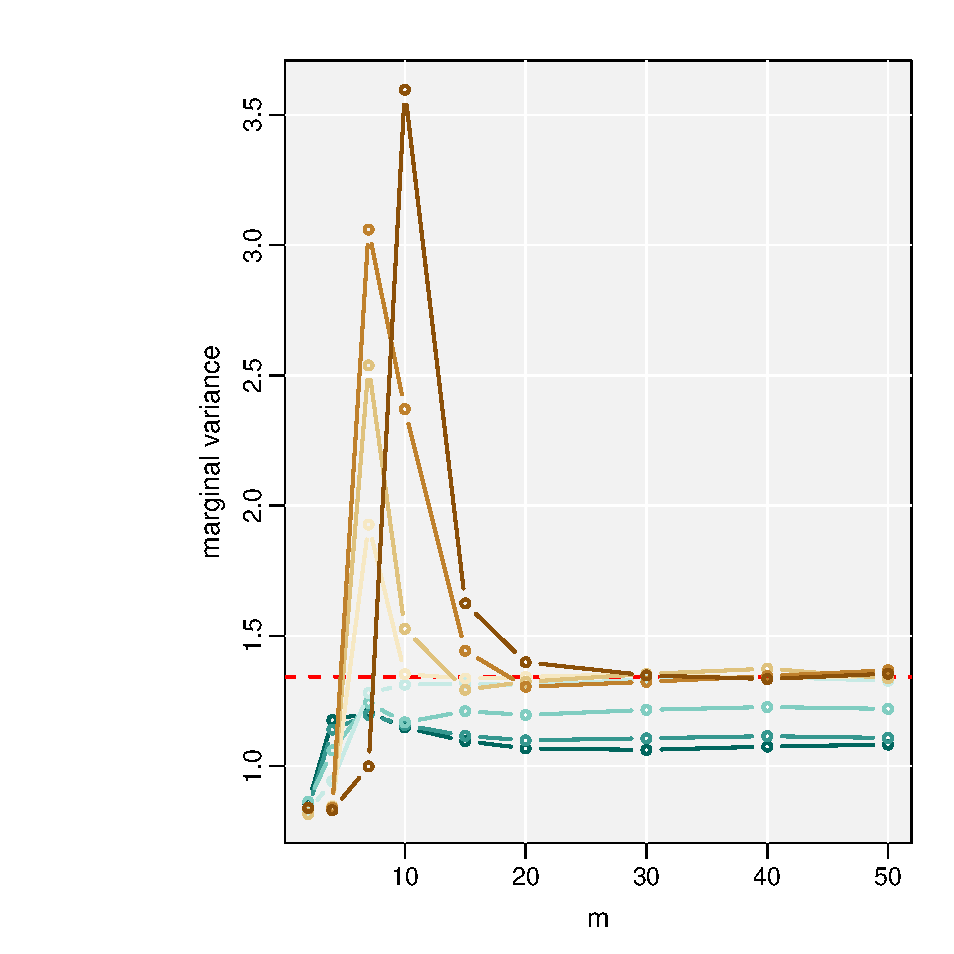
\includegraphics[scale=0.4]{fig6_magnitud_vs_J.pdf}}
\caption{Estimated lengthscale and marginal variance parameters of the proposed HSGP models and the regular GP model. (left) Estimated lengthscales vs the number of basis functions $m$ and for different values of the boundary factor $c$. (right) Estimated marginal variance vs the number of basis functions $m$ and for different values of the boundary factor $c$.}
  \label{fig6_lscale_vs_J}
\end{figure}


Additionally, there exit a relation of the number of basis functions $m$ and the boundary factor $c$ with the lengthscale $\ell$ of the function. Figure \ref{fig3_lscale_vs_J_vs_c_part1} collects how these three factors relate each other in relation to the performance of the approximation evaluated using eq. (\ref{diff_covs}). On the X-axis of this plot is placed the lengthscale of the process normalized by the half-range of the data $\ell/S$. The countour lines gather the boundary factor $c$. And the Y-axis represents the number of basis functions. Thus, this figure give us, for a certain GP function with lengthscale $\ell$ and given a boundary factor $c$, the minimum number of basis functions needed to achieve a close approximation in terms of satisfying eq. (\ref{diff_covs}). Alternatively, this figure could also be read as the minimum boundary factor $c$ that we should use given a number of basis functions, for certain GP function with certain lengthscale. And also this figure could also be read as the minimum functional lengthscales that can be closely approximated given a number of basis functions and a boundary factor. This figure basically collects the behaviour of the HSGP model as a function of the lengthscale, number of basis functions and boundary factor:

$\bullet$ As the lengthscale of the function increases, the boundary factor and the number of basis functions needed for the approximation decrease.

$\bullet$ There is a minimum boundary factor under which a close approximation never is going to be achieved (The contour lines have an end in function of the lengthscale). This statement match with one of the behaviour recognized in Figure \ref{fig6_lscale_vs_J} where were a minimum value for the boundary factor under which a close approximation will never be achieved.

$\bullet$ The lower the boundary factor, the fewer basis functions and the smaller lengthscales that are suitable to be fitted. 

$\bullet$ This plot serves as a diagnosis tool in the sense that if a estimated lengthscale is lower than that minimum that the figure bring us, given certain number of basis functions and certain boundary factor, means that the number of basis functions should be increased or the boundary factor decreased. On the other hand, if the lengthscale is bigger than that generated by the figure means that the approximation should be close enough.

Figure \ref{fig3_lscale_vs_J_vs_c_part1} is useful for the user to know the suitable values for the number of basis functions $m$ and the boundary factor $c$ to approximate certain process characterized by its lengthscale. This Figure will allow us to optimize computations which depends on the number of basis functions. Starting from some guess of the lengthscale of the process and knowing the range of the input data which we are interested in, the user can do a few iterative adjustments to obtain an optimal fit. This figure also provides a diagnosis tool of the fit by comparing a actual estimated lengthscale to that the figure bring. 

\begin{figure}[H]
\centering
\subfigure{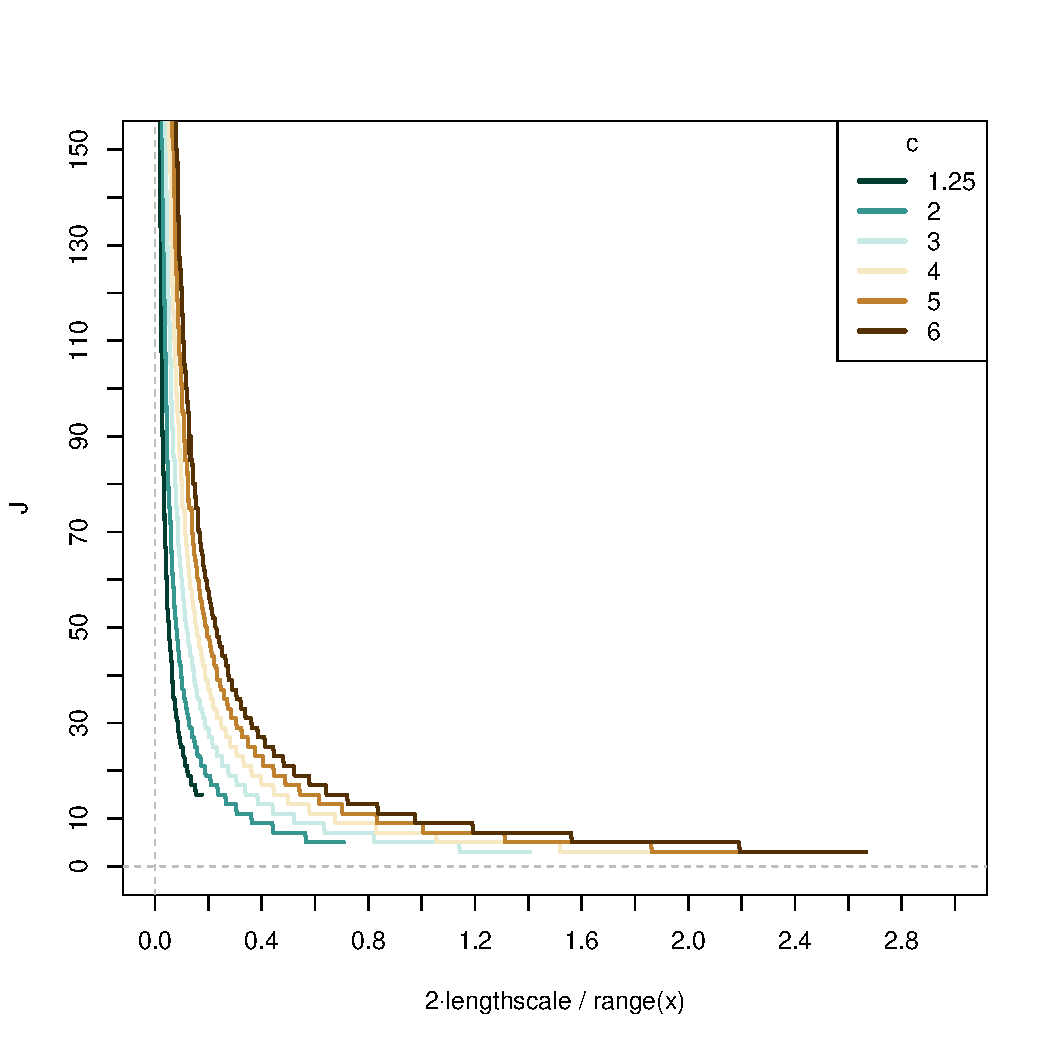
\includegraphics[scale=0.4]{fig3_lscale_vs_J_vs_c_part1.pdf}}
\subfigure{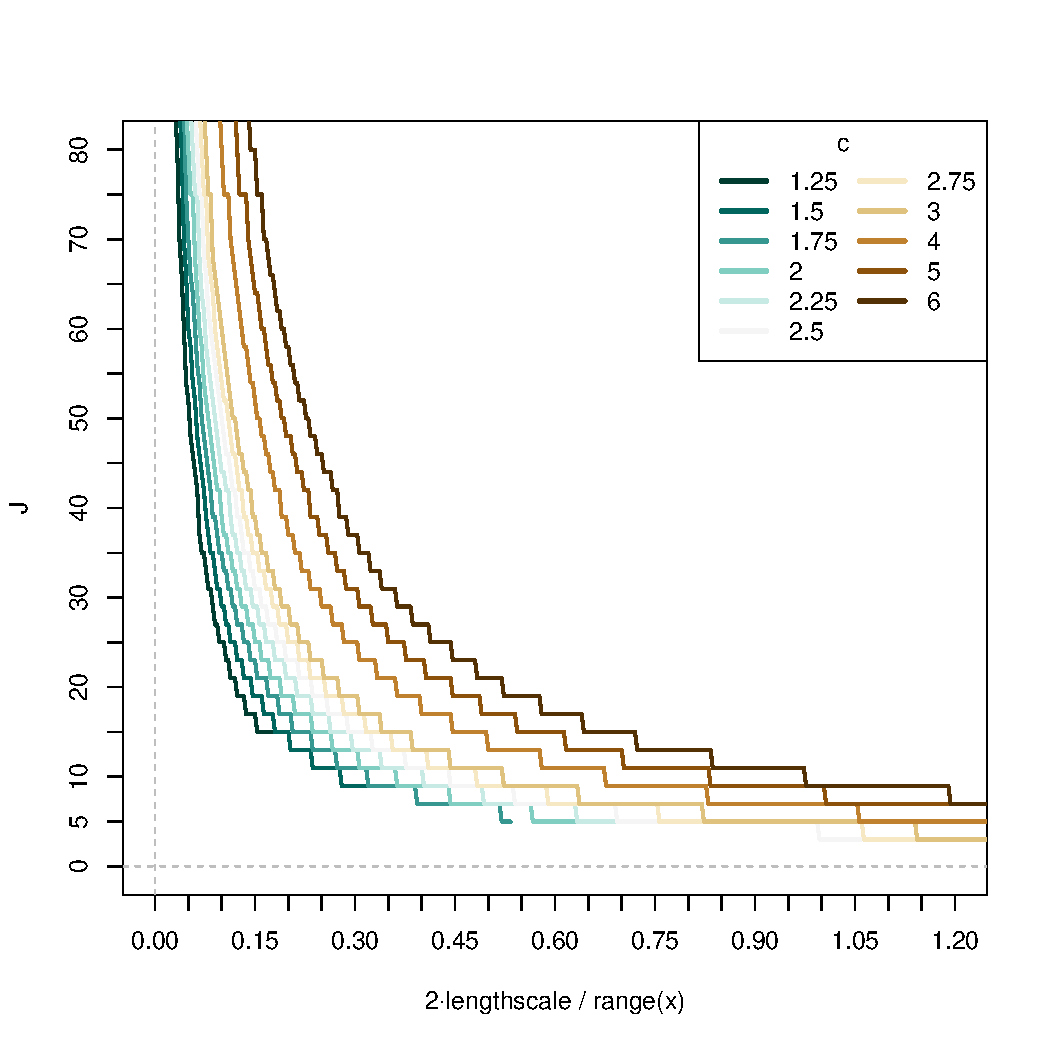
\includegraphics[scale=0.4]{fig3_lscale_vs_J_vs_c_part2.pdf}}
\caption{Relation between the minimum number of basis functions $m$, the lengthscale normalized by the half-range of the data ($\frac{\ell}{S}$), and the boundary factor $c$ ($c = \frac{L}{S}$).}
  \label{fig3_lscale_vs_J_vs_c_part1}
\end{figure}

If we look back to the conclusions drawn from Figures \ref{fig5_MSE_vs_J} and \ref{fig6_lscale_vs_J} where 10 basis functions and a boundary factor of 1.5 would be enough to closely approximate a function with normalized lengthscale equal to 0.3, we can recognize that these conclusions also matches the conclusion brought from Figure \ref{fig3_lscale_vs_J_vs_c_part1}.

\subsection{Comparative analysis between the lengthscales estimated by a regular GP model and approximate GP model}

We make a comparative analysis between the lengthscales estimated by the regular GP model and the approximate GP model in several datasets with different "wigglyness" (or lengthscales). Basically, comparing the lengthscales we can recognize if an approximation is close enough to the regular GP. We contrast these results with the information brought from Figure \ref{fig3_lscale_vs_J_vs_c_part1}.

For this analysis, we fit the regular GP model and the approximate GP model on different datasets. These datasets consists of noisy draws from a GP prior model with a squared exponential covariance function with different lengthscale. Different number of basis functions are used to fit the approximate GP model. The boundary factor is set in every case to a right and optimal choice. Figure \ref{fig7_varing_lscale} shows the posterior means of the regular GP model and the approximate GP model with different number of basis functions, for every dataset.

\begin{figure}
\centering
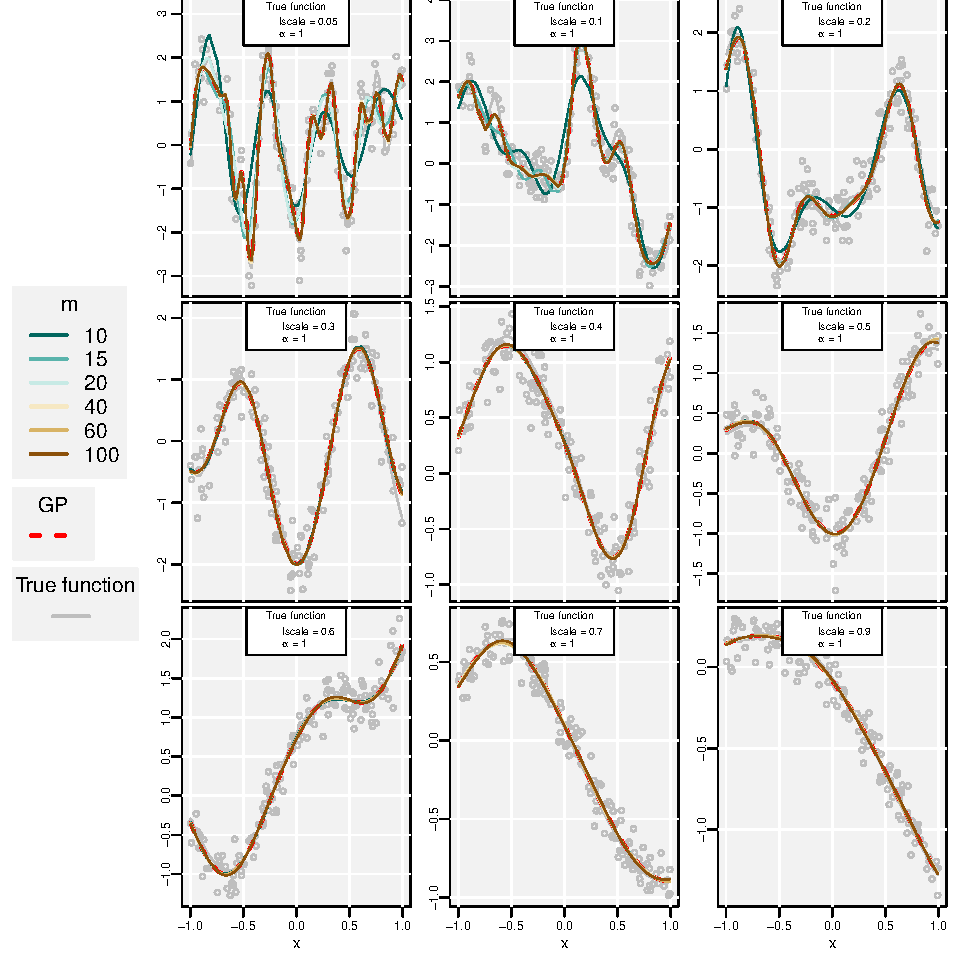
\includegraphics[width=\textwidth]{fig7_varing_lscale.pdf}
\caption{Posterior means of the regular GP and approximate GP models fitted over different datasets with different lengthscales.}
  \label{fig7_varing_lscale}
\end{figure}

The comparative analysis between the lengthscales, estimated by a regular GP model and an approximate GP model in the different datasets with different lengthscales, is shown in Figure \ref{fig8_Tlscale_vs_Elscale}. In the X-axes of the plots, the true lengthscales of the data-generative functions for every dataset scenario are represented. In the Y-axes, the estimated lengthscales for the regular GP and approximate GP models are represented. Different comparisons are made using different number of basis functions in the approximate GP model. Let's assume that the boundary factor was properly set in every case. The dashed black line represents the minimum lengthscales that can be closely approximate given the number of basis functions and the boundary factor, according to Figure \ref{fig3_lscale_vs_J_vs_c_part1}. Figure \ref{fig9_MSE_varing_lscale} shows the SRMSE of the approximate GP model, computed against the regular GP model, as a function of the lengthscale and number of basis functions.

We can appreciate an agreement between Figures \ref{fig8_Tlscale_vs_Elscale} and \ref{fig9_MSE_varing_lscale} except for small lengthscales and long lengthscales. Very small changes on small lengthscales, which might not be appreciated in Figure \ref{fig8_Tlscale_vs_Elscale}, can have big effects on the posteriors and therefore high SRMSE. On the other side, big changes on long lengthscales, which might clearly appreciated in Figure \ref{fig8_Tlscale_vs_Elscale}, might result in similar posterior and therefore a small SRMSE.

\begin{figure}
\centering
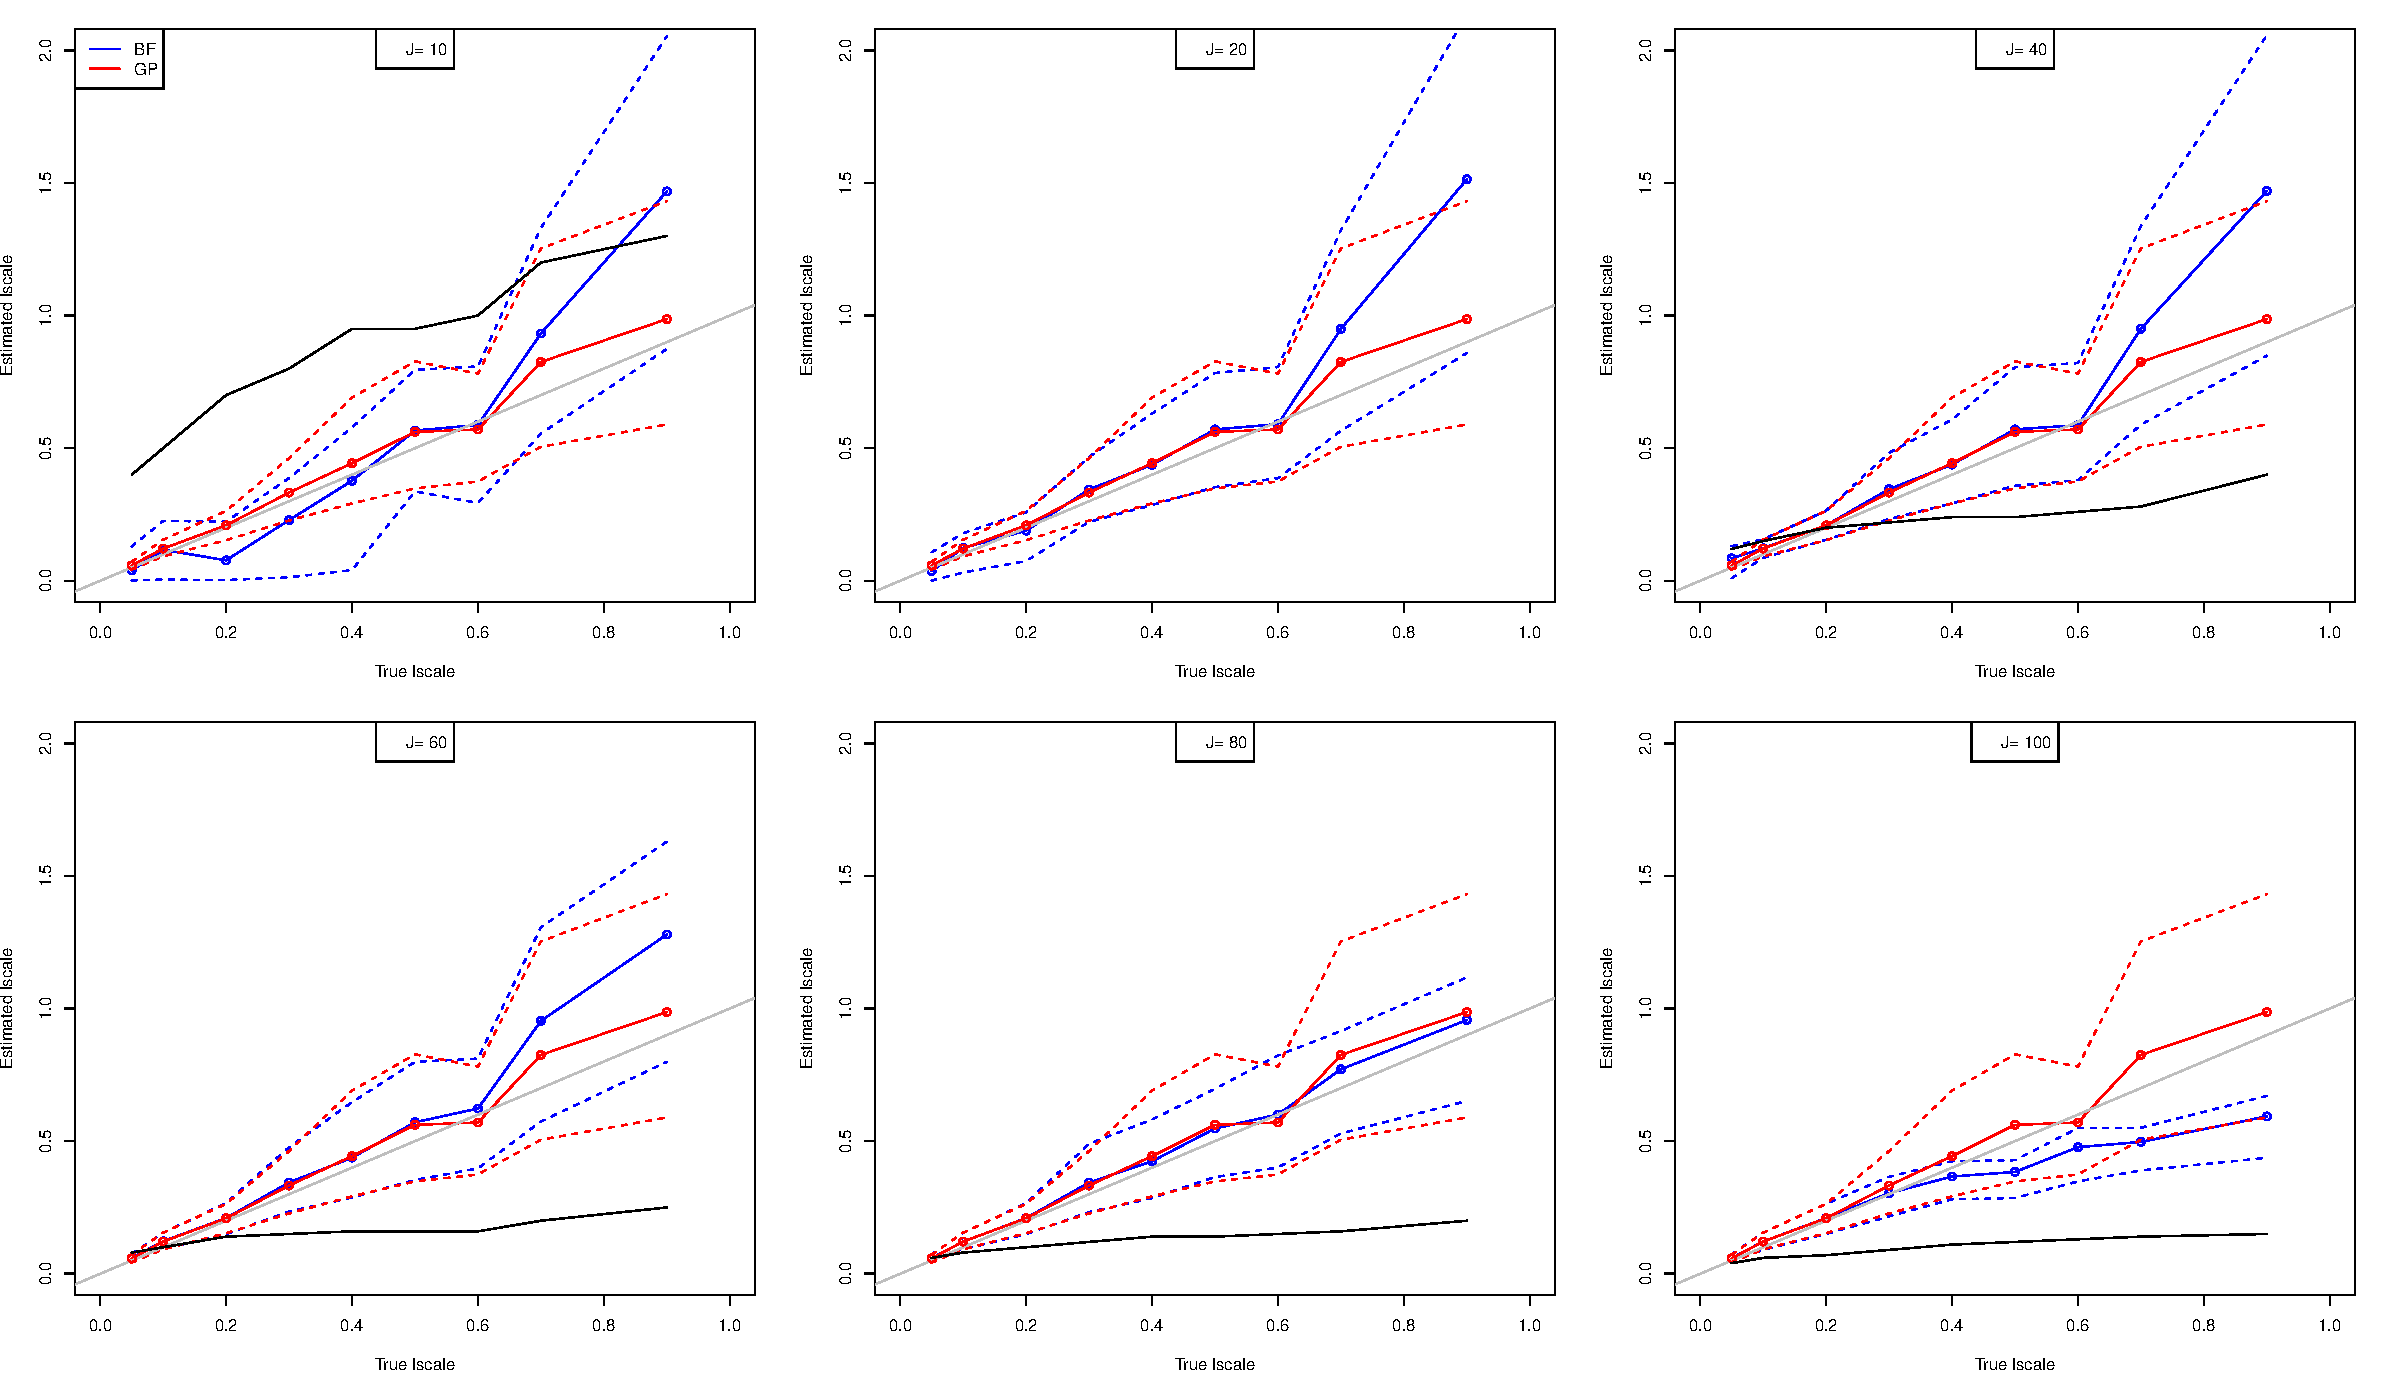
\includegraphics[width=\textwidth]{fig8_Tlscale_vs_Elscale.pdf}
\caption{True lengthscales versus estimated lengthscales of the different realizations of datasets using different number of basis functions. }
  \label{fig8_Tlscale_vs_Elscale}
\end{figure}

\begin{figure}[H]
\centering
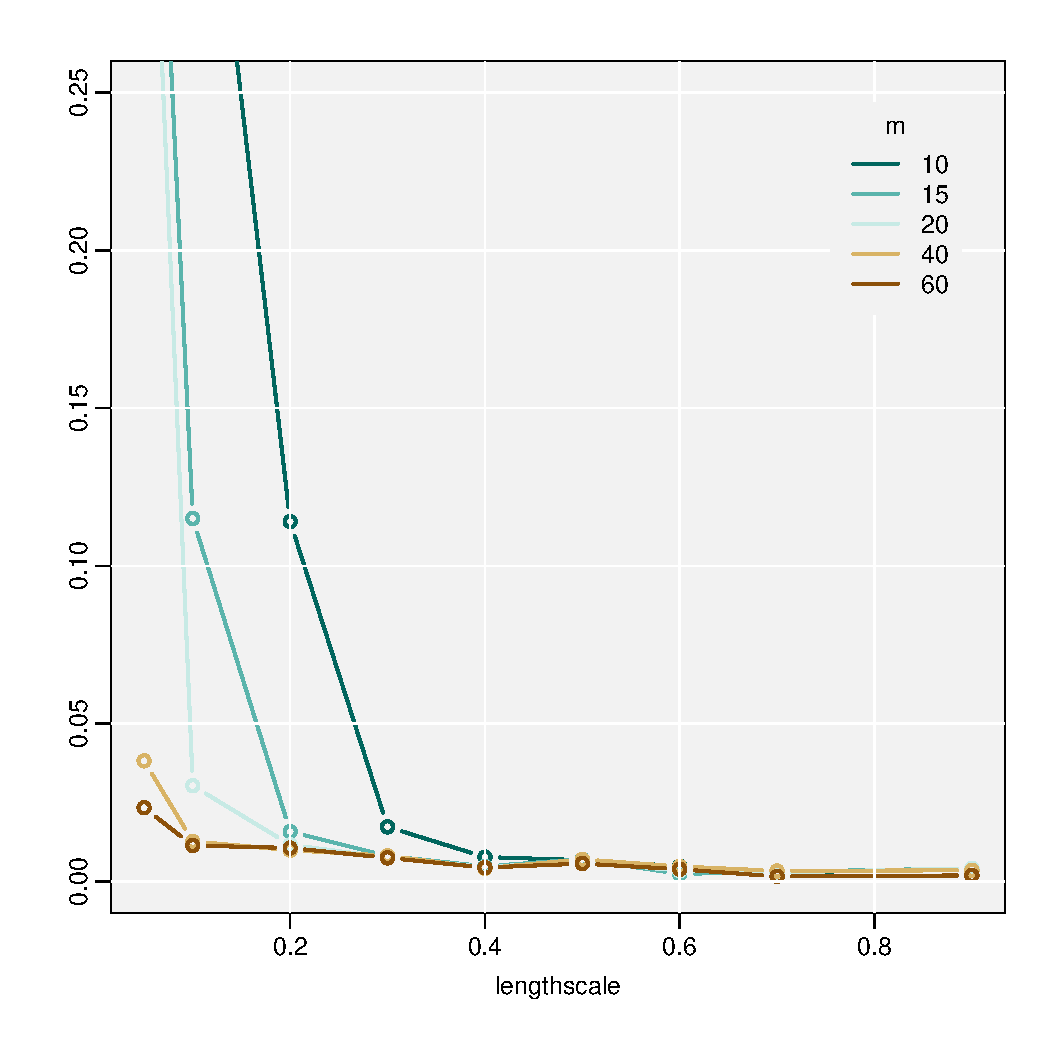
\includegraphics[scale=0.45]{fig9_MSE_varing_lscale.pdf}
\caption{SMSE of the approximate GP model for the different datasets with different wiggly effects and number of basis functions.}
  \label{fig9_MSE_varing_lscale}
\end{figure}


\vspace{3mm}
\section{Univariate examples}\label{sec:gp_examples1D}


\subsection{Simulated data}

This example consist of a simulated dataset with 250 draws values from a Gaussian process prior with a Matern covariance function (a Matern with 3/2 degrees of freedom) and inputs $\{\mathbf{x}_i\}_{i=1}^{250} \in \{-1,1\} \subset {\rm I\!R}$. The hyperparameters, marginal variance $\alpha$ and lengthscale $\ell$, of this GP prior were set to 1 and 0.15, respectively. The Gaussian noise $\sigma$ added to these draws was set to 0.2.

The regular GP model for fitting this simulated dataset $\mathbf{y}$ can be written as follows,
%
\begin{eqnarray}\label{eq:latentgp_simudata1}
\begin{split}
\mathbf{y} &= f(\mathbf{x}) + \boldsymbol{\epsilon} \\
\boldsymbol{\epsilon} &\sim \mathcal{N}(0, \sigma^2  \mathbf{I}) \\
f(\mathbf{x}) &\sim \mathcal{GP}(0, k(\mathbf{x}, \mathbf{x}', \theta)),
\end{split}
\end{eqnarray}

\noindent The previous formulation corresponds to the latent form where $f(\mathbf{x})$ represents the functional model underlying the noisy data and modeled by a GP prior with a Matern covariance function $k$ (4). $\mathbf{I}$ represents the identity matrix. Saying that the function values $f(\mathbf{x})$ follows a GP model is equivalent to say that $f(\mathbf{x})$ are multivariate Gaussian distributed with covariance matrix $K$, where the element $K_{ij}$ is formed by evaluating the covariance function $k(\mathbf{x}_i,\mathbf{x}_j,\theta)$ at input values $\mathbf{x}_i$ and $\mathbf{x}_j$.
 
A more computationally efficient formulation of a GP model with Gaussian likelihood, and for probabilistic inference using sampling methods such as HMC, would be the marginalized form of the latent GP model in (\ref{eq:latentgp_simudata1}),
%
\begin{equation*}\label{eq:marginalizedgp_simudata1}
\mathbf{y} \sim \mathcal{N}(0, K + \sigma^2 \mathbf{I} )
\end{equation*}

\noindent where the function values $f(\mathbf{x})$ have been integrated out, yielding a lower-dimensional parameter space over which to do inference, reducing time of computation and improving the sampling and the effective number of samples.

In the HSGP model, the covariance function $k$ is approximated as (\ref{approxcov}),
%
\begin{equation*}
k(x,x') \approx \sum_{j}^{m}S(\sqrt{\lambda_j}) \phi_j(x) \phi_j(x'),
\end{equation*} 

\noindent with the spectral density $S$ (3),
%
\begin{eqnarray*}
S(w)&=& 4\alpha^2 \frac{\sqrt{3}}{\ell}^{3}(\frac{3}{\ell^2} + \omega^2)^{-2},  
\end{eqnarray*}

\noindent and the latent function values $f(\mathbf{x)}$ are approximated as (\ref{approxf}),
%
\begin{equation*}
f(x) \approx \sum_{j}^m \left( S(\sqrt{\lambda_j})\right)^{1/2} \phi_j(x) \beta_j, \nonumber
\end{equation*}

In order to do model comparison, in addition to the regular GP model and HSGP model, an splines-based model is also fitted using the Thin Plate Regression Splines approach in \cite{wood2003thin} and implemented in the R-package \textit{mgcv}. A Bayesian approach is used to fit this splines model using the R-package \textit{brms}.

For the HSGP model we use $m=80$ basis functions and a boundary factor $c=1.2$. For the splines model we use 80 knots or basis in the model.

Figure \ref{fig10_Posteriors_exI} shows the posteriors distributions of the three models, the regular GP, the HSGP and the splines, jointly with the true data-generative function and the noisy observations. The right and left extremes and three small regions around the middle of the plot correspond to out-of-sample or test data which have not been taking part on training the models. The test data have been plotted in Figure \ref{fig10_Posteriors_exI} with crosses and the training data with circles. The test data located at the extremes of the plot are used for assessing model extrapolation, and the test data located in the middle are used for assessing model interpolation.

\begin{figure}[H]
\centering
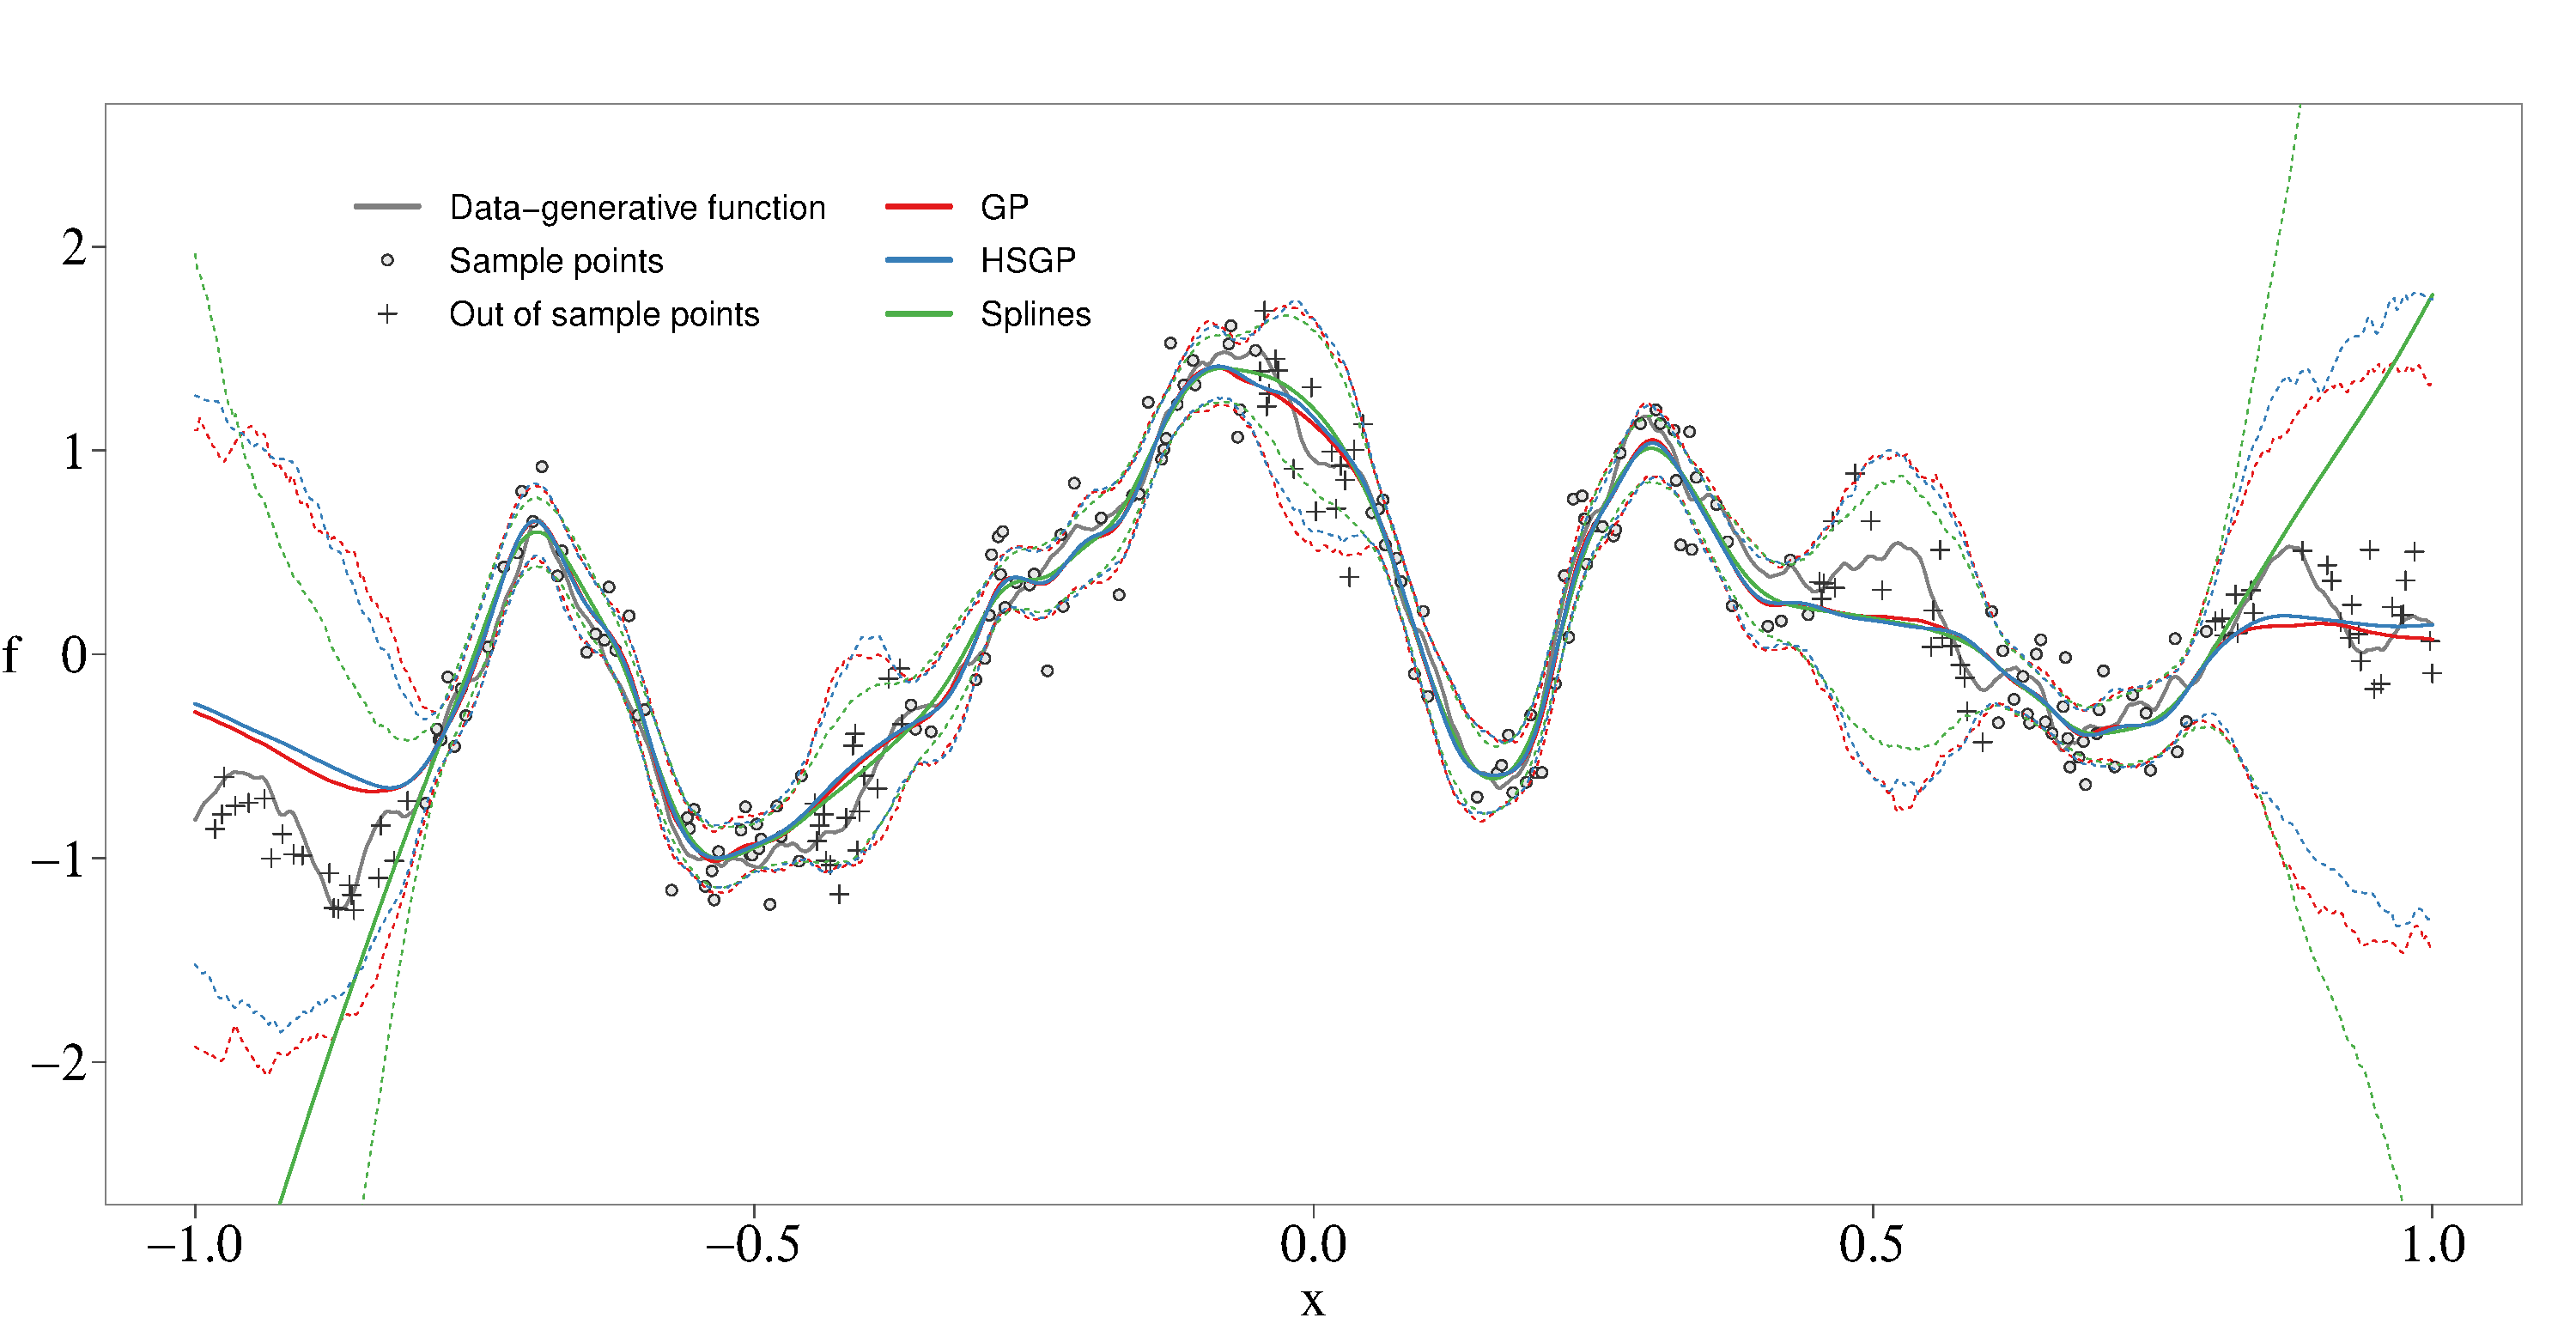
\includegraphics[scale=0.35]{fig10_Posteriors_exI.pdf}
\caption{Posterior distributions of the proposed HSGP model, the regular GP model, and the Splines model.}
  \label{fig10_Posteriors_exI}
\end{figure}

Figure \ref{fig11_MSE_exI_inter} shows the  standardized root mean squared error (SRMSE), for interpolation and extrapolating data, as a function of the number of basis functions and knots. For this, different models with different number of basis functions for the HSGP model and different number of knots for the splines model have been formulated and fitted on this data. The SRMSE is computed against the true function. Model interpolation has been assessed either using the test data for interpolating and the training data. From Figures \ref{fig10_Posteriors_exI} and \ref{fig11_MSE_exI_inter}, it can be seen a close approximation of the HSGP model to the regular GP model, for interpolating and extrapolating data. However, the splines model does not extrapolate data properly. For interpolation both models show roughly similar performance.

\begin{figure}[H]
\centering
\subfigure{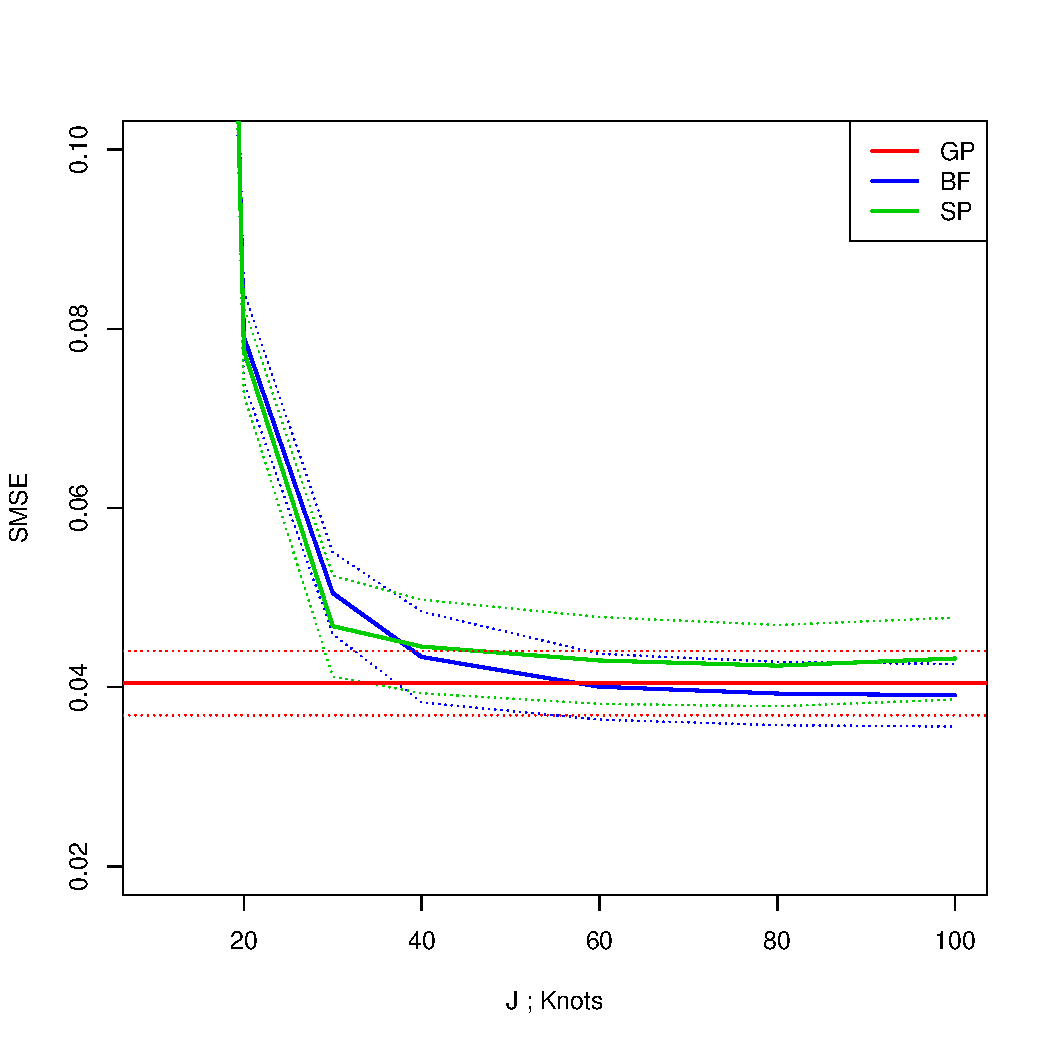
\includegraphics[scale=0.350]{fig11_MSE_exI_inter.pdf}}
\subfigure{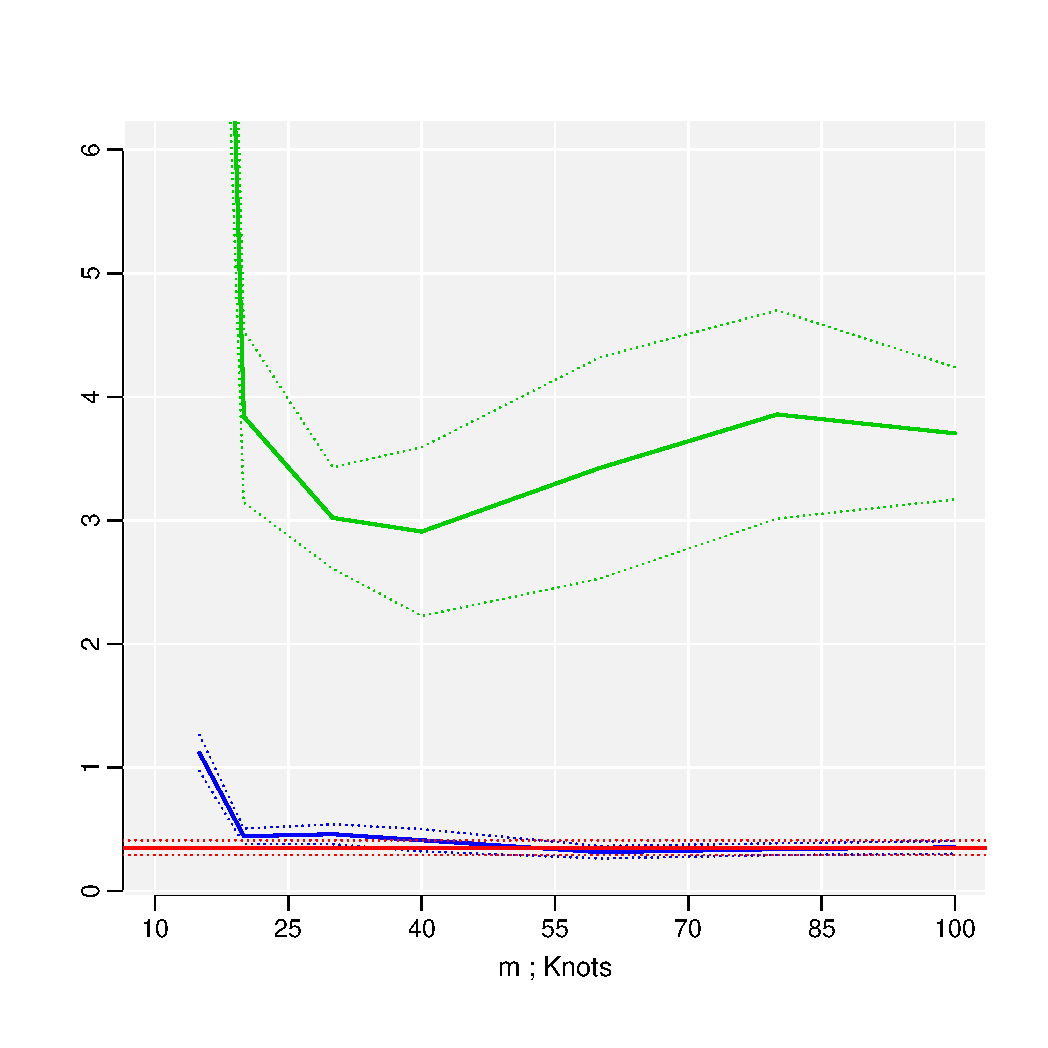
\includegraphics[scale=0.350]{fig11_MSE_exI_extra.pdf}}
\caption{Standardized mean square error (SMSE) of the different methods against the true function. (left) SMSE for interpolation. (right) SMSE for extrapolation}
  \label{fig11_MSE_exI_inter}
\end{figure}

\subsection{Gay data}\label{sec:gay_data}
This data set relates the proportion of support for same-sex marriage to the age. The data consists of 74 binomial observations per age group $i$ ($i=1,\cdots,74$), with the observation of the amount of people $y_i$ supporting same-sex marriage from a population $n_i$ per age group. 

The observational model for the observed number of people $y_i$ supporting same-age marriage per age group $i$ is a binomial model with the total number of people $n_i$ per age group and the probability $p_i$ per age group as model parameters,
%
\begin{equation*}
y_i \sim \text{Binomial}(p_i, n_i).
\end{equation*}

\noindent The total number of people per age group $n_i$ is a known quantity and the goal is to estimate the same-sex support probability $p_i$ per age group $i$ or mean number of support people per age group $i$. The probability $p_i$ is related to the Gaussian process latent values $f(\mathbf{x})$ with age values $\mathbf{x}=\{x_i\}_{i=1}^{74}$ as inputs, through the logit function,
%
\begin{eqnarray*} \label{eq:gpprior_gay}
p_i &=& \text{logit}(f(x_i)) \nonumber \\
f(\mathbf{x}) &\sim& \mathcal{GP}(0, k(\mathbf{x},\mathbf{x}', \theta)
\end{eqnarray*}

\noindent with a squared exponential covariance function $k$ (2). 

In the HSGP model the covariance function is approximated as in eq. (\ref{approxcov}) with the square exponential spectral density in eq. (6), and the latent function $f(\mathbf{x})$ as in eq. (\ref{approxf}). 

In order to do model comparison, in addition to the regular GP model and HSGP model, an splines-based model is also fitted using the Thin Plate Regression Splines approach in \cite{wood2003thin} and implemented in the R-package \textit{mgcv}. A Bayesian approach is used to fit this splines model using the R-package \textit{brms}.

For the HSGP model we use $m=20$ basis functions and a boundary factor $c=1.5$. For the splines model we use 20 knots or basis in the model.

Figure \ref{fig12_Posteriors_gaydata} shows the posteriors distributions of the three models, the regular GP, the HSGP and the splines, jointly with the true data-generative function and the noisy observations. The HSGP model posterior shown in the figure corresponds to 20 basis functions and a boundary factor of 1.5. For the spline posterior shown in the figure, it correspond to a 20 knots. Two small sets of observations have been used as test data, plotted as crosses in the Figure. 

\begin{figure}[H]
\centering
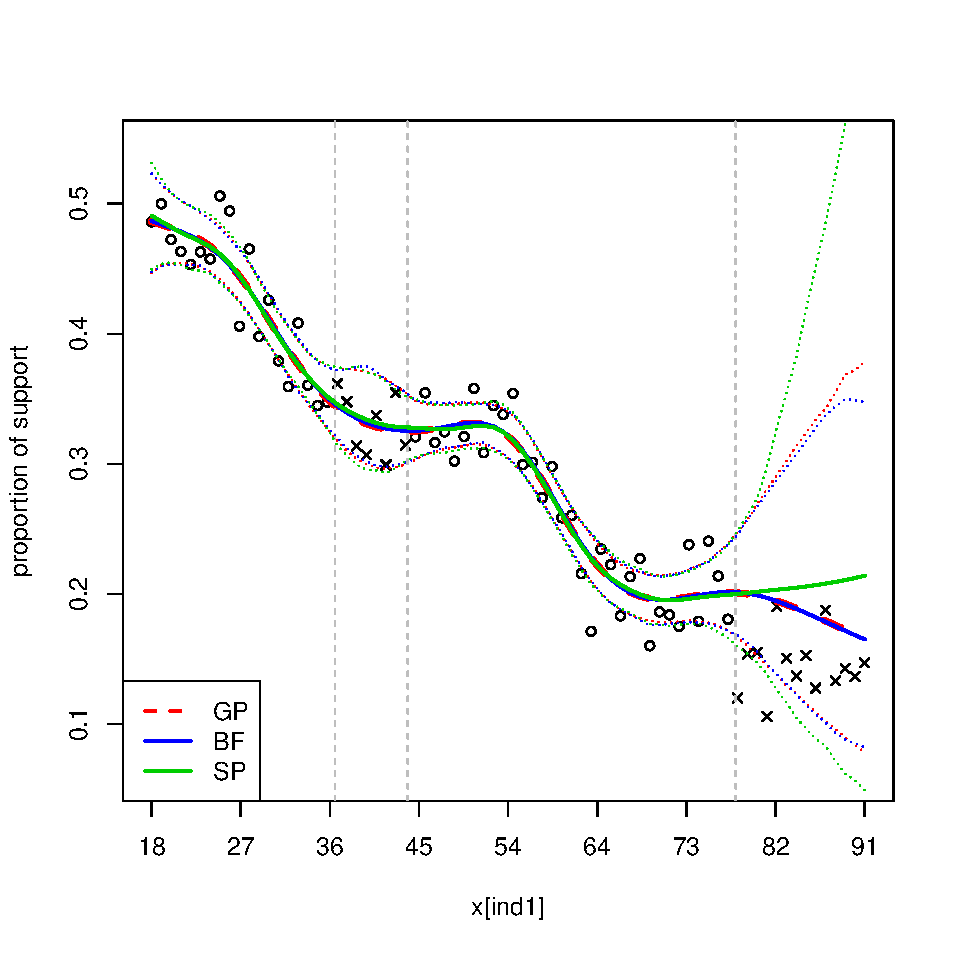
\includegraphics[scale=0.50]{fig12_Posteriors_gaydata.pdf}
\caption{Posterior distributions of the proposed HSGP model, the regular GP model, and the Splines model.}
  \label{fig12_Posteriors_gaydata}
\end{figure}

For the HSGP model, different models with different number of basis functions and boundary factors have been used. The root mean square errors (RMSE) for every one of these models have been computed and plotted as a function of the number of basis functions and the boundary factor in Figure \ref{fig13_MSE_train_BF_gaydata}, for training (left) and test (right) data. In this case, the RMSE has been computed against the regular GP model. The expected patterns of the approximation in function of the number of basis function and boundary factor are recognized: as the boundary factor increases, more basis functions are needed.

\begin{figure}[H]
\centering
\subfigure{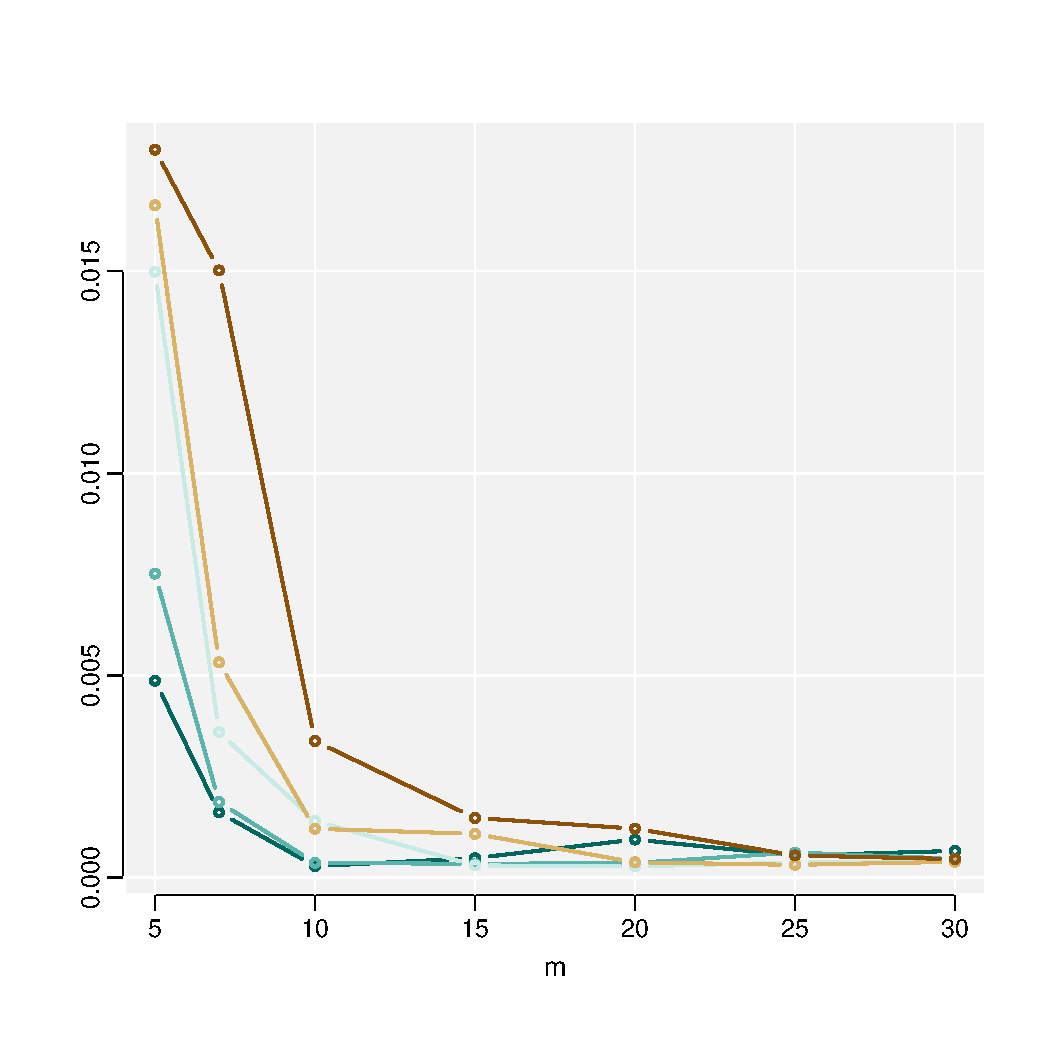
\includegraphics[scale=0.40]{fig13_MSE_train_BF_gaydata.pdf}}
\subfigure{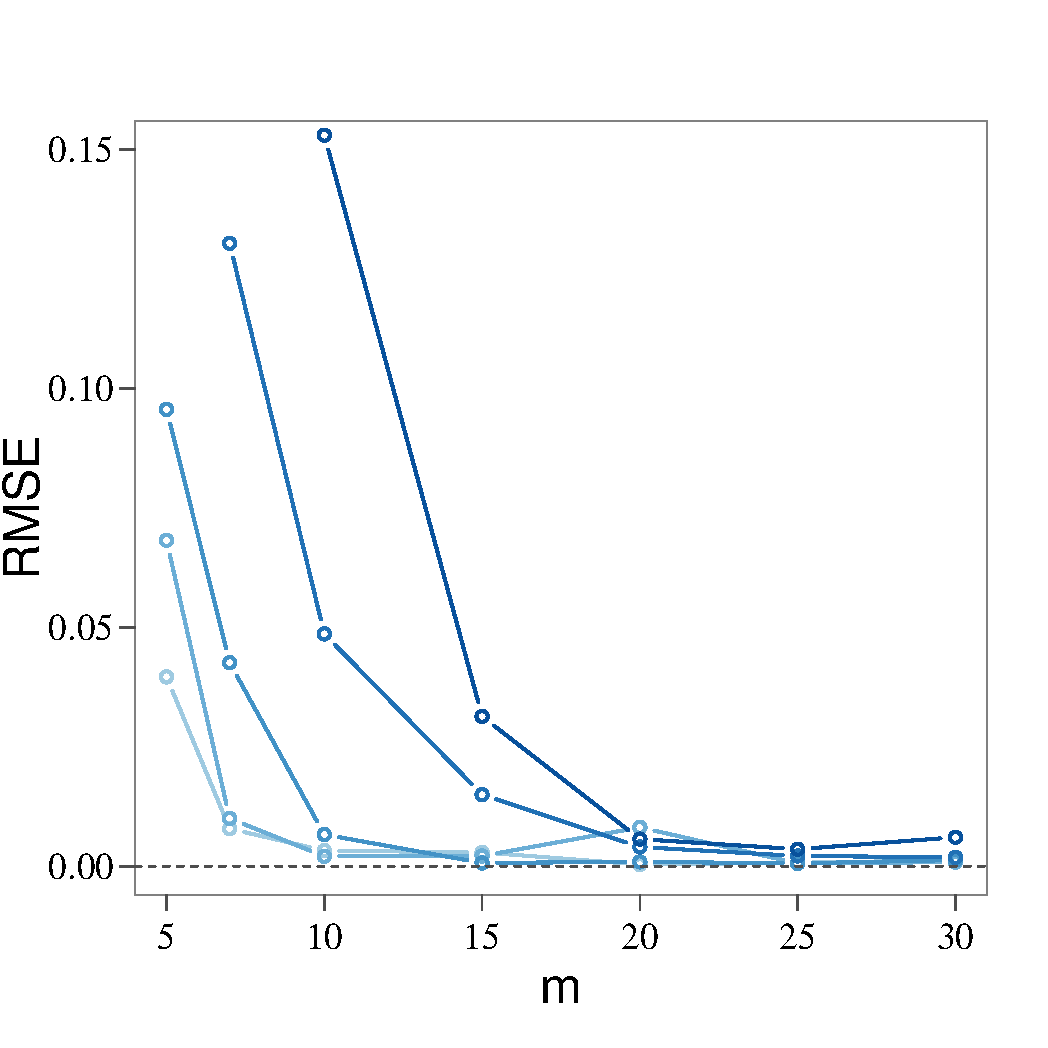
\includegraphics[scale=0.40]{fig13_MSE_pred_BF_gaydata.pdf}}
\caption{Mean square error (MSE) of the different methods against the true function. (left) MSE for training data. (right) MSE for test data.}
  \label{fig13_MSE_train_BF_gaydata}
\end{figure}

Figure \ref{fig14_MSE_train_gaydata} shows the RMSE of the different models, regular GP, HSGP and splines, against the actual data, for training and test data. Again we can see how the splines models does not extrapolate data properly.

\begin{figure}[H]
\centering
\subfigure{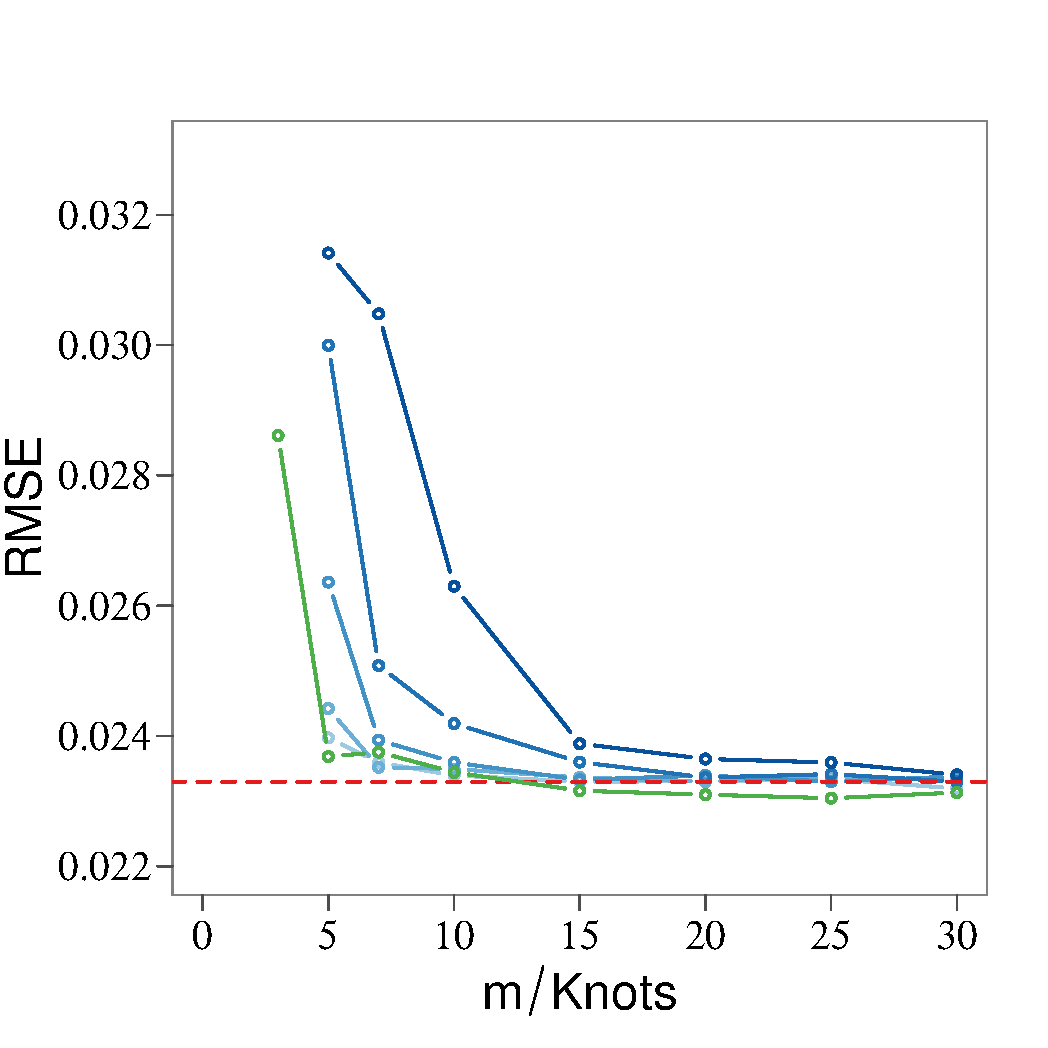
\includegraphics[scale=0.40]{fig14_MSE_train_gaydata.pdf}}
\subfigure{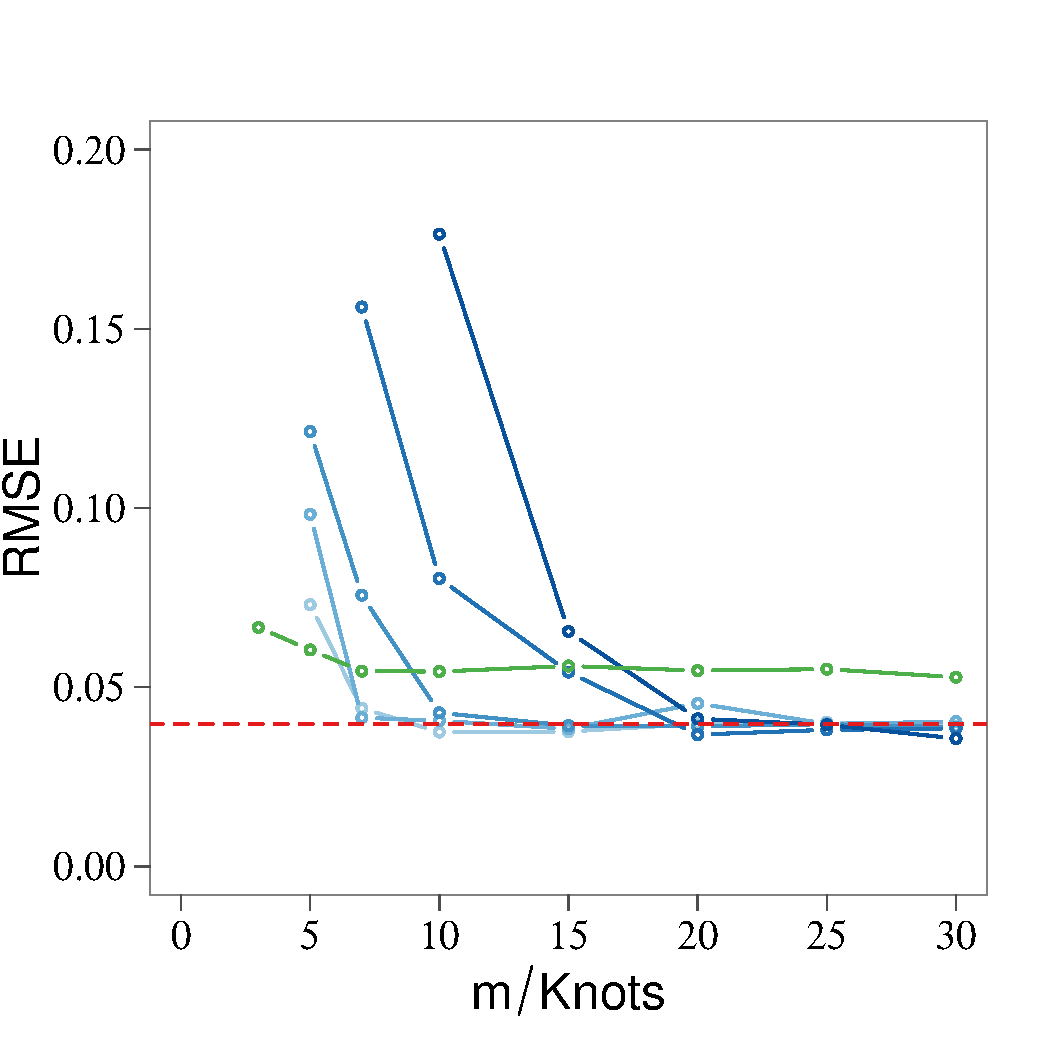
\includegraphics[scale=0.40]{fig14_MSE_pred_gaydata.pdf}}
\caption{Mean square error (MSE) of the different methods against the true function. (left) MSE for training data. (right) MSE for test data.}
  \label{fig14_MSE_train_gaydata}
\end{figure}


\subsection{Case II: Birthday data}\label{sec:bf_caseIII}

\vspace{3mm}
\section{Multivariate examples}\label{sec:gp_examplesMulti}
\subsection{Simulated data}\label{sec:bf_toyexampleMulti}
\subsection{Case III: Diabetes data}\label{sec:bf_caseIV}
\subsection{Case IV: Leukemia data}\label{sec:bf_caseV}
\subsection{Case V: Land use spatio-temporal classification task}\label{sec:bf_caseVII}

\vspace{3mm}
\appendix

\section{Related work}

The GP prior entails an $O(n^3)$ complexity that is computationally intractable for many practical problems, and this problem especially becomes severe when we want to conduct inference using sampling methods. To overcome this scaling problem several schemes have been proposed. One approach is to partition the data set into separate groups \citep{snelson2007local, urtasun2008sparse} and performing local inference in each partition. Other global approach is to build a low-rank approximation to the covariance matrix of the complete data based around 'inducing variables' \citep{quinonero2005unifying,bui2017unifying}. Other global approach make use of basis functions to approximate the covariance function. In \cite{snelson2007local} the authors conduct an approach that combines the idea of local and global approaches.

The literature contains many parametric models that approximate Gaussian process behaviours; for example \cite{bui2014tree} included  tree-structures in the approximation for extra scalability, and \cite{moore2015gaussian} combined local Gaussian
processes with Gaussian random fields.

\subsection{Inducing points methods}

The approach based on inducing points employs a small set of pseudo data points to summarise the actual data. The storage requirements are reduced to $O(nm)$ and complexity to $O(nm^2)$, where $m < n$. Some of these methods have been reviewed in \cite{rasmussen2006gaussian}, and \cite{quinonero2005unifying} provide a unifying view of these methods based on approximate generative methods. From a spectral point of view, several of these methods (e.g., SOR, DTC, VAR, FIC) can be interpreted as modfications to the so-called Nystr{\"o}m method (see \cite{arthur1979baker} and \cite{williams2001using}), a scheme for approximating the eigenspectrum. These methods are basically based on choosing a set of $m$ inducing inputs $x_u$ and scaling the corresponding eigendecomposition of their corresponding covariance matrix $K_{u,u}$ to match that of the actual covariance. 

This scheme was originally introduced to the GP context by \cite{williams2001using}. As discussed by \cite{quinonero2005unifying}, the Nystr\"om method by \cite{williams2001using} does not correspond to a well-formed probabilistic model. However, several methods modifying the inducing point approach are widely used. The Subset of Regressors (SoR) \citep{smola2001sparse} method uses the Nystr\"om approximation scheme and a finite linear-in-the-parameters model for approximating the whole (training and test) covariance function, whereas the sparse Nystr\"om method \citep{williams2001using} only replaces the training data covariance matrix. The SoR method is based on a degenerate prior which produces unreasonable predictive uncertainties, which is a general problem of linear models (for more details see \cite{rasmussen2006gaussian}). 

The Deterministic Training Conditional (DTC) method \citep{ro2001sparse,seeger2003fast}) retains the true covariance for the training data, but uses the approximate cross-covariances between training and test data, which reverse the problem of nonsensical predictive uncertainties. However, since the covariances for training and test cases are computed differently, this method results not to actually be a Gaussian process. This method was presented as Projected Latent Variables (PLV) in \cite{seeger2003fast} and Projected Process Approximation (PPA) in \cite{rasmussen2006gaussian}. 

The Variational Approximation (VAR) \citep{titsias2009variational} suggests a variational approach which provides an objective function for optimizing the selection of inducing points. This basically modifies the DTC method by an additional trace term in the likelihood that comes from the variational bound.  \cite{hensman2013gaussian} extended this idea by introducing additional variational parameters to enable stochastic variational inference \citep{hoffman2013stochastic}, achieving a more computationally scalable bound which allows GPs to be fitted to millions of data.

The Fully Independent (Training) Conditional (FIC) \citep{quinonero2005unifying} method originally introduced as Sparse Pseudo-Input GP by \cite{snelson2006sparse} is also based on the Nystr\"om approximation, where they allow the pseudo-point input locations to be optimised by maximising the new model's marginal likelihood whose covariance is parameterized by the locations of an active set not constrained to be a subset of the training and test data.

More recently Bui et. al (2017) revisit the inducing points-based sparse approximation methods, in which all the necessary approximation is performed at inference time, rather than at the modelling time. The new framework is built on standard methods for approximate inference (variational-free-inference, EP and Power EP methods). 

In practice, the inducing points-based sparse approximation methods works reasonable well in cases where the field is relatively smooth. \cite{vanhatalo2010approximate}
propose the use of compactly supported covariance function in conjunction with sparse approximations to model both short and long range correlations.

\cite{wilson2015kernel} introduce a new unifying framework for inducing point methods, called structured kernel interpolation (SKI). This framework improves the scalability and accuracy of fast kernel approximations through kernel interpolation, and naturally combines the advantages of inducing point and structure exploiting for scalability (such as Kronecker \citep{saatcci2012scalable} or Toeplitz \citep{cunningham2008fast}) approaches.

The number of inducing points or their locations are crucial in order to capture the correlation structure. For a discussion on the effects of the inducing points, see \cite{vanhatalo2010approximate}. This behavior applies to all the methods from the Nystr\''om family.

This kind of 'projected process' approximation has also been discussed by e.g. \cite{banerjee2008gaussian}.


\subsection{Basis function methods}

The spectral analysis and series expansions of Gaussian processes has a long history. A classical result (see, e.g, \cite{loeve1977probability,trees1968detection,adler1981geometry,cramer2013stationary}, and references therein) is that the covariance function can be approximated with a finite truncation of Mercer series and the approximation is guaranteed to converge to the exact covariance function when the number of terms is increased. 

Another related classical connection is to the works in the relationship of spline interpolation and Gaussian process priors \citep{wahba1978improper,kimeldorf1970correspondence,wahba1990spline}. In particular, it is well-known (see, e.g., \cite{wahba1990spline}) that spline smoothing can be seen as Gaussian process regression with a specific choice of covariance function. The relationship of the spline regularization with Laplace operators then leads to series expansion representations that are closely related to the approximations considered here. 

Random Fourier Features \citep{rahimi2008random,rahimi2009weighted} is a method for approximating kernels. The approximate kernel has a finite basis function expansion.


The Sparse Spectrum GP is based on a sparse approximation to the frequency domain representation of a GP \citep{lazaro2010sparse,quia2010sparse}, where the spectral representation of the covariance function is used. This model is a stationary sparse GP that can approximate any desired stationary full GP. However, as argued by the authors, this option does not converge to the full GP and can suffer from overfitting to the training data. \citep{gal2015improving} sought to improve the model by integrating out, rather than optimizing the frequencies. Gal and Turner derived a variational approximation that made use of a tractable integral over the frequency space. The result is an  algorithm that suffers less overfitting than the Sparse Spectrum GP, yet remains flexible.

While Sparse Spectrum GP is based on a sparse spectrum, the reduced-rank method proposed in this paper aims to make the spectrum as ‘full’ as possible at a given rank.

Recently \citep{hensman2017variational} presented a variational Fourier feature approximation for Gaussian processes that was derived for the Mat{\'e}rn class of kernels, where the approximation structure is set up by a low-rank plus diagonal structure. They combine the variational methodology with Fourier based approximations.

In spatial statistics similar approaches are called low-rank models \citep{diggle2007springer}. The low rank models assume that the Gaussian field is a linear combination of $m$ basis functions. The type of an approximation depends on the basis functions used. Familiar examples include spectral representation \citep{diggle2007springer,paciorek2007computational,paciorek2007bayesian} and splines \citep{wood2003thin}. 

Recent Splines models can reproduce the Matern family of covariance functions, however our approach can reproduce basically all of the stationary covariance functions.


\section{Contributions of the method}

This work is based on the novel method developed by \cite{solin2018hilbert} for reduced-rank approximations of GP models. This method is based on interpreting the covariance function as the kernel of a pseudo-differential operator and approximating it using Hilbert space methods. This results in a reduced-rank approximation for the covariance function. This method has some nice features:

\vspace{2mm}
$\bullet$ It has an attractive computational cost as this basically turns the regular GP model into a lineal model.

\vspace{2mm}
$\bullet$ In a fully Bayesian inference framework using sampling methods, the proposed approximate GP model has a computational complexity of $O(nm+m)$ in every step of the HMC method. In addition, the computation of the automatic differentiation to compute the gradients in this linear model scales $O(n)$?, an operation that must be computed in every step of the HMC method.

\vspace{2mm}
$\bullet$ Using maximizing marginal likelihood methods, the proposed model has a overall complexity of $O(nm^2)$. After this, evaluating the marginal likelihood and marginal likelihood gradients is an $O(m^3)$ operation in every step of the optimizer. (Arno's paper, pag. 7)

\vspace{2mm}
$\bullet$ The parameter posterior distribution in this approximate GP model is $m$-dimensional ($m<<n$) which helps the use of GP priors as latent functions. especially when sampling methods for inference are used. GP prior as latent functions is needed in generalized models.

In regular GPs and other approximate GP models and Splines models these features do not have so nice properties:

\vspace{2mm}
$\bullet$ In a regular GPs, the main computational complexity comes from the inversion of the covariance matrix which is in general a $O(n^3)$ operation. This operation has to be computed at every step of the HMC or optimizer.

\vspace{2mm}
$\bullet$ In regular GPs, the parameter posterior distributions is $N$-dimensional. It is known that when $N$ is of medium or large size there is high correlation between the $N$-dimensional latent function and the hyperparameters of the GP prior.

\vspace{2mm}
$\bullet$ In conventional sparse GP approximations, although the rank of the GP is reduced considerably to the number of inducing points, this still needs to do the autodiff and covariance matrix inversion.

\vspace{2mm}
$\bullet$ The Splines models are also a sort of basis functions expansion model, then the computational demands are similar to that in this approach. However in Splines models the lengthscale hyperparameter tend to be fixed and then the fit is covered by the magnitude parameter. In that sense, Splines models tend to loose the useful interpretation of the lengthscale parameter.



\section{Contributions of our work}

As said above the proposed method was already developed by \cite{solin2018hilbert} where they fully develop, describe and generalize the methodology. Though, they do not put much effort in describing and analyzing the relation among the key factors of the box size (or boundary condition), the number of basis functions, and the smoothness or roughness of the function. The performance and accuracy of the method are directly related with the number of basis functions and the box size. At the same time, successful values for these two factors depend on the smoothness or roughness of the process to be modeled. The time of computation is mainly dependent on the number of basis functions. Our main contributions to this recently developed methodology for low-rank GP model by \cite{solin2018hilbert} goes around these aspects.

\vspace{2mm}
$\bullet$ Firstly, clear summarized formulae of the method for the univariate and multivariate cases is presented. 

\vspace{2mm}
$\bullet$ We investigate the relations going on among these factors, the number of basis functions, the box size, and the lengthscale of the functions.

\vspace{2mm}
$\bullet$ We make recommendations for the values of these factors based on the recognized relations among them. We provide useful graphs of these relations that will help the users to improve performance and save time of computation.

\vspace{2mm}
$\bullet$ We also diagnose if the chosen values for the number of basis functions and the box size are adequate to fit to the actual data.

\vspace{2mm}
$\bullet$ We describe the generalization of the method to the multidimensional case.

\vspace{2mm}
$\bullet$ We implement the approach in a fully probabilistic framework and for the Stan programming probabilistic software.

\vspace{2mm}
$\bullet$ We show several illustrative examples, simulate and real datasets, of the performance of the model, and accompanied by their Stan codes.

 
%\vspace{3mm}
%A summary of the formulae of the method for the univariate and multivariate cases is presented. The number of basis functions used in the approach and the value for the boundary condition of the model are two factors of main importance in practical applications. The number of basis functions is directly related to the accuracy of the approximation but also to the computation demands. Also exist a relation among the number of basis functions, the specified values for the boundary condition, and the performance of the approach.  Finally, the approach is applied in several illustrative study cases and accompanied by their Stan codes.

\section{Spectral densities of stationary covariance functions}

The covariance function of a stationary process, that is function of $\boldsymbol{\tau}=\mathbf{x-x'}$ can be represented as the Fourier transform of a positive finite measure ($Bochner's theorem$). 

\vspace{0.2cm}
\textit{(Bochner’s theorem) A complex-valued function $k$ on ${\rm I\!R}^D$ is the covariance function of a weakly stationary mean square continuous complex valued random process on ${\rm I\!R}^D$ if and only if it can be represented as}
%
\begin{equation}
k(\boldsymbol{\tau})= \int_{{\rm I\!R}^D} e^{2\pi i \mathbf{s} \cdot \mathbf{\tau}} d\mu(\boldsymbol{\tau}), \nonumber 
\end{equation}

\textit{where $\mu$ is a positive finite measure.} 

\vspace{0.2cm}
If the measure $\mu$ has a density, it is known as the spectral density $S(\omega)$ of the covariance function, and the covariance function and the spectral density are Fourier duals, known as the Wiener-Khintchine theorem. It gives the following relations:

\begin{eqnarray}
k(\boldsymbol{\tau})&=& \int S(\mathbf{s}) e^{2\pi i \mathbf{s} \cdot \boldsymbol{\tau}} d\mathbf{s}  \nonumber \\
%
S(\mathbf{s})&=& \int k(\boldsymbol{\tau}) e^{-2\pi i \mathbf{s} \cdot \boldsymbol{\tau}} d\mathbf{s}  \nonumber
\end{eqnarray}

\section{Approximate the covariance function using Hilbert space methods}

Associated to each covariance function $k(\mathbf{x},\mathbf{x}')$ we can also define a covariance operator $\mathcal{K}$ as follows:
%
\begin{equation}
\mathcal{K} f(\mathbf{x}) = \int k(\mathbf{x},\mathbf{x}') f(\mathbf{x}') d\mathbf{x}'.
\end{equation} 

Assuming that the spectral density function $S(\cdot)$ is regular enough, then it can be represented as a polynomial expansion:
%
\begin{equation}
S(\mathbf{w})=a_0+a_1\mathbf{w}^2+a_2(\mathbf{w}^2)^2+a_1(\mathbf{w}^2)^3+\cdots
\end{equation}


If the negative Laplace operator $-\nabla^2$ is defined as the covariance operator of the covariance function $k$,

\begin{equation}
-\nabla^2 f(\mathbf{x}) = \int k(\mathbf{x},\mathbf{x}') f(\mathbf{x}') d\mathbf{x}',
\end{equation} 

\noindent then the covariance function can be represented as 

\begin{equation}
k(\mathbf{x},\mathbf{x}')= \sum_j \lambda_j \phi_j(\mathbf{x}) \phi_j(\mathbf{x}'),
\end{equation}

\noindent where $\{\lambda_j\}_{j=1}^{\infty}$ and $\{\phi_j(x)\}_{j=1}^{\infty}$ are the set of eigenvalues and eigenvectors, respectively, of the Laplacian operator. Namely, they satisfy the following eigenvalue problem in the compact subset $x \in \{-L,L\}$ and with the Dirichlet boundary condition (another boundary condition could be used as well):
%
\begin{eqnarray}
-\nabla^2 \phi_j(x)&=&\lambda \phi_j(x), \hspace{1cm}  x\in \{-L,L\} \nonumber \\ 
\phi_j(x)&=&0, \hspace{2cm} x\notin \{-L,L\}.
\end{eqnarray}  

a series expansion of eigenvalues and eigenfunctions 


\section{Example of generalization to the multivariate case}

Next, as an example we show the matrix $\mathbb{S}$ and eigenfunctions and eigenvalues for a $two$-dimensional input vector $\mathbf{x}=\{\mathbf{x}_1,\mathbf{x}_2\}$ ($D=2$) and three eigenfunctions and eigenvalues $(J=3)$ for every dimension. The number of new multidimensional eigenfunctions $\phi^{\ast}_j$ and eigenvalues $\lambda^{\ast}_j$ is $J^D=3^2=9$ ($j=\{1,\cdots,J^D\}$). The matrix $\mathbb{S}\in {\rm I\!R}^{9 \times 2}$ is
%
\begin{eqnarray}
\mathbb{S}=
\left[ {\begin{array}{cc}
1 & 1 \nonumber \\
1 & 2 \\
1 & 3 \\
2 & 1 \\
2 & 2 \\
2 & 3 \\
3 & 1 \\
3 & 2 \\
3 & 3
\end{array} } \right]
\end{eqnarray} 

\noindent and the multidimensional eigenfunctions and eigenvalues
%
\begin{eqnarray}
\phi^{\ast}_1(\mathbf{x}) = \phi_{1}(\mathbf{x}_1) \cdot \phi_{1}(\mathbf{x}_2)  \hspace{2cm}
%
\boldsymbol{\lambda}^{\ast}_1 = \{\lambda_{1}(\mathbf{x}_1), \lambda_{1}(\mathbf{x}_2)\}  \nonumber \\
%
\phi^{\ast}_2(\mathbf{x}) = \phi_{1}(\mathbf{x}_1) \cdot \phi_{2}(\mathbf{x}_2)  \hspace{2cm}
%
\boldsymbol{\lambda}^{\ast}_2 = \{\lambda_{1}(\mathbf{x}_1), \lambda_{2}(\mathbf{x}_2)\} \nonumber \\
%
\phi^{\ast}_3(\mathbf{x}) = \phi_{1}(\mathbf{x}_1) \cdot \phi_{3}(\mathbf{x}_2) \hspace{2cm}
%
\boldsymbol{\lambda}^{\ast}_3 = \{\lambda_{1}(\mathbf{x}_1), \lambda_{3}(\mathbf{x}_2)\}  \nonumber \\
%
\phi^{\ast}_4(\mathbf{x}) = \phi_{2}(\mathbf{x}_1) \cdot \phi_{1}(\mathbf{x}_2)  \hspace{2cm}
%
\boldsymbol{\lambda}^{\ast}_4 = \{\lambda_{2}(\mathbf{x}_1), \lambda_{1}(\mathbf{x}_2)\}  \nonumber \\
%
\phi^{\ast}_5(\mathbf{x}) = \phi_{2}(\mathbf{x}_1) \cdot \phi_{2}(\mathbf{x}_2)  \hspace{2cm}
%
\boldsymbol{\lambda}^{\ast}_5 = \{\lambda_{2}(\mathbf{x}_1), \lambda_{2}(\mathbf{x}_2)\}  \nonumber \\
%
\phi^{\ast}_6(\mathbf{x}) = \phi_{2}(\mathbf{x}_1) \cdot \phi_{3}(\mathbf{x}_2)  \hspace{2cm}
%
\boldsymbol{\lambda}^{\ast}_6 = \{\lambda_{2}(\mathbf{x}_1), \lambda_{3}(\mathbf{x}_2)\}  \nonumber \\
%
\phi^{\ast}_7(\mathbf{x}) = \phi_{3}(\mathbf{x}_1) \cdot \phi_{1}(\mathbf{x}_2)  \hspace{2cm}
%
\boldsymbol{\lambda}^{\ast}_7 = \{\lambda_{3}(\mathbf{x}_1), \lambda_{1}(\mathbf{x}_2)\}  \nonumber \\
%
\phi^{\ast}_8(\mathbf{x}) = \phi_{3}(\mathbf{x}_1) \cdot \phi_{2}(\mathbf{x}_2)  \hspace{2cm}
%
\boldsymbol{\lambda}^{\ast}_8 = \{\lambda_{3}(\mathbf{x}_1), \lambda_{2}(\mathbf{x}_2)\}  \nonumber \\
%
\phi^{\ast}_9(\mathbf{x}) = \phi_{3}(\mathbf{x}_1) \cdot \phi_{3}(\mathbf{x}_2)  \hspace{2cm}
%
\boldsymbol{\lambda}^{\ast}_9 = \{\lambda_{3}(\mathbf{x}_1), \lambda_{3}(\mathbf{x}_2)\}  \nonumber
\end{eqnarray}

Now, we show another example where different number of eigenfunctions and eigenvalues are used for every dimension. We consider a three-dimensional ($D=3$) input space, and sets of $J_{1}=2$, $J_{2}=2$ and $J_{3}=3$ eigenfunctions and eigenvalues for the first, second and third dimensions, respectively. The number of new multidimensional eigenfunctions $\phi^{\ast}$ and eigenvalues $\lambda^{\ast}$ is $J_{1}\cdot J_{2}\cdot J_{3}=2\cdot 2\cdot 3=12$. The matrix $\mathbb{S}\in {\rm I\!R}^{12 \times 3}$ is
%
\begin{eqnarray}
\mathbb{S}=
\left[ {\begin{array}{ccc}
1 & 1 & 1 \nonumber \\
1 & 1 & 2 \\
1 & 1 & 3 \\
1 & 2 & 1 \\
1 & 2 & 2 \\
1 & 2 & 3 \\
2 & 1 & 1 \\
2 & 1 & 2 \\
2 & 1 & 3 \\
2 & 2 & 1 \\
2 & 2 & 2 \\
2 & 2 & 3 
\end{array} } \right]
\end{eqnarray} 

\noindent and the multidimensional eigenfunctions and eigenvalues
%
\begin{eqnarray}
\phi^{\ast}_1= \phi_{1}(\mathbf{x}_1) \cdot \phi_{1}(\mathbf{x}_2) \cdot \phi_{1}(\mathbf{x}_3) \hspace{1.5cm} \boldsymbol{\lambda}^{\ast}_1= \{\lambda_1(\mathbf{x}_1), \lambda_1(\mathbf{x}_2), \lambda_1(\mathbf{x}_3)\} \nonumber \\
%
\phi^{\ast}_2= \phi_{1}(\mathbf{x}_1) \cdot \phi_{1}(\mathbf{x}_2) \cdot \phi_{2}(\mathbf{x}_3) \hspace{1.5cm} \boldsymbol{\lambda}^{\ast}_2= \{\lambda_1(\mathbf{x}_1), \lambda_1(\mathbf{x}_2), \lambda_2(\mathbf{x}_3)\} \nonumber \\
%
\phi^{\ast}_3= \phi_{1}(\mathbf{x}_1) \cdot \phi_{1}(\mathbf{x}_2) \cdot \phi_{3}(\mathbf{x}_3) \hspace{1.5cm} \boldsymbol{\lambda}^{\ast}_3= \{\lambda_1(\mathbf{x}_1), \lambda_1(\mathbf{x}_2), \lambda_3(\mathbf{x}_3)\} \nonumber \\
%
\phi^{\ast}_4= \phi_{1}(\mathbf{x}_1) \cdot \phi_{2}(\mathbf{x}_2) \cdot \phi_{1}(\mathbf{x}_3) \hspace{1.5cm} \boldsymbol{\lambda}^{\ast}_4= \{\lambda_1(\mathbf{x}_1), \lambda_1(\mathbf{x}_2), \lambda_1(\mathbf{x}_3)\} \nonumber \\
%
\phi^{\ast}_5= \phi_{1}(\mathbf{x}_1) \cdot \phi_{2}(\mathbf{x}_2) \cdot \phi_{2}(\mathbf{x}_3) \hspace{1.5cm} \boldsymbol{\lambda}^{\ast}_5= \{\lambda_1(\mathbf{x}_1), \lambda_1(\mathbf{x}_2), \lambda_2(\mathbf{x}_3)\} \nonumber \\
%
\phi^{\ast}_6= \phi_{1}(\mathbf{x}_1) \cdot \phi_{2}(\mathbf{x}_2) \cdot \phi_{3}(\mathbf{x}_3) \hspace{1.5cm} \boldsymbol{\lambda}^{\ast}_6= \{\lambda_1(\mathbf{x}_1), \lambda_1(\mathbf{x}_2), \lambda_3(\mathbf{x}_3)\} \nonumber \\
%
\phi^{\ast}_7= \phi_{2}(\mathbf{x}_1) \cdot \phi_{1}(\mathbf{x}_2) \cdot \phi_{1}(\mathbf{x}_3) \hspace{1.5cm} \boldsymbol{\lambda}^{\ast}_7= \{\lambda_2(\mathbf{x}_1), \lambda_2(\mathbf{x}_2), \lambda_1(\mathbf{x}_3)\} \nonumber \\
%
\phi^{\ast}_8= \phi_{2}(\mathbf{x}_1) \cdot \phi_{1}(\mathbf{x}_2) \cdot \phi_{2}(\mathbf{x}_3) \hspace{1.5cm} \boldsymbol{\lambda}^{\ast}_8= \{\lambda_2(\mathbf{x}_1), \lambda_2(\mathbf{x}_2), \lambda_2(\mathbf{x}_3)\} \nonumber \\
%
\phi^{\ast}_9= \phi_{2}(\mathbf{x}_1) \cdot \phi_{1}(\mathbf{x}_2) \cdot \phi_{3}(\mathbf{x}_3) \hspace{1.5cm} \boldsymbol{\lambda}^{\ast}_9= \{\lambda_2(\mathbf{x}_1), \lambda_2(\mathbf{x}_2), \lambda_3(\mathbf{x}_3)\} \nonumber \\
%
\phi^{\ast}_{10}= \phi_{2}(\mathbf{x}_1) \cdot \phi_{2}(\mathbf{x}_2) \cdot \phi_{1}(\mathbf{x}_3) \hspace{1.5cm} \boldsymbol{\lambda}^{\ast}_{10}= \{\lambda_2(\mathbf{x}_1), \lambda_2(\mathbf{x}_2), \lambda_1(\mathbf{x}_3)\} \nonumber \\
%
\phi^{\ast}_{11}= \phi_{2}(\mathbf{x}_1) \cdot \phi_{2}(\mathbf{x}_2) \cdot \phi_{2}(\mathbf{x}_3) \hspace{1.5cm} \boldsymbol{\lambda}^{\ast}_{11}= \{\lambda_2(\mathbf{x}_1), \lambda_2(\mathbf{x}_2), \lambda_2(\mathbf{x}_3)\} \nonumber \\
%
\phi^{\ast}_{12}= \phi_{2}(\mathbf{x}_1) \cdot \phi_{2}(\mathbf{x}_2) \cdot \phi_{3}(\mathbf{x}_3) \hspace{1.5cm} \boldsymbol{\lambda}^{\ast}_{12}= \{\lambda_2(\mathbf{x}_1), \lambda_2(\mathbf{x}_2), \lambda_3(\mathbf{x}_3)\} \nonumber
\end{eqnarray}


\vspace{2mm}
\section*{Acknowledgment}

\bibliographystyle{biom}
\bibliography{references}


\end{document}



###########
#######
Next we show a little example of how to construct the new set of eigenfunctions and eigenvalues with input vector $\mathbf{x}=\{\mathbf{x}_1,\mathbf{x}_2\}$ in a two-dimensional input space ($D=2$) and three eigenfunctions and eigenvalues $(J=3)$ for every dimension. As a result we obtain sets of $J^D=3^2=9$ new eigenfunctions $\phi^{\ast}$ and eigenvalues $\lambda^{\ast}$. The eigenfunctions $\phi^{\ast}$ are the product combination of the unidimensional eigenfunctions $\phi$, and eigenvalues $\lambda^{\ast}$ is the $D$-vector of unidimensional eigenvalues $\lambda$:




\begin{eqnarray}
\phi^{\ast}_1(\mathbf{x}) = \phi_{1}(\mathbf{x}_1) \cdot \phi_{1}(\mathbf{x}_2) &=& \sqrt{\tfrac{1}{L_1}} \text{sin}\left(\sqrt{\lambda_1}(\mathbf{x}_1+L_1)\right) \cdot \sqrt{\tfrac{1}{L_2}} \text{sin}\left(\sqrt{\lambda_1}(\mathbf{x}_2+L_2)\right) \nonumber \\
%
\boldsymbol{\lambda}^{\ast}_1 = \{\lambda_{1}(\mathbf{x}_1), \lambda_{1}(\mathbf{x}_2)\} &=& \{ \left(\tfrac{1\pi}{2L_1}\right)^2, \left(\tfrac{1\pi}{2L_2}\right)^2 \} \nonumber \\
%
\phi^{\ast}_2(\mathbf{x}) = \phi_{1}(\mathbf{x}_1) \cdot \phi_{2}(\mathbf{x}_2) &=& \sqrt{\tfrac{1}{L_1}} \text{sin}\left(\sqrt{\lambda_1}(\mathbf{x}_1+L_1)\right) \cdot \sqrt{\tfrac{1}{L_2}} \text{sin}\left(\sqrt{\lambda_2}(\mathbf{x}_2+L_2)\right) \nonumber \\
%
\boldsymbol{\lambda}^{\ast}_2 = \{\lambda_{1}(\mathbf{x}_1), \lambda_{2}(\mathbf{x}_2)\} &=& \{ \left(\tfrac{1\pi}{2L_1}\right)^2, \left(\tfrac{2\pi}{2L_2}\right)^2 \} \nonumber \\
%
\phi^{\ast}_3(\mathbf{x}) = \phi_{1}(\mathbf{x}_1) \cdot \phi_{3}(\mathbf{x}_2) &=& \sqrt{\tfrac{1}{L_1}} \text{sin}\left(\sqrt{\lambda_1}(\mathbf{x}_1+L_1)\right) \cdot \sqrt{\tfrac{1}{L_2}} \text{sin}\left(\sqrt{\lambda_3}(\mathbf{x}_2+L_2)\right) \nonumber \\
%
\boldsymbol{\lambda}^{\ast}_3 = \{\lambda_{1}(\mathbf{x}_1), \lambda_{3}(\mathbf{x}_2)\} &=& \{ \left(\tfrac{1\pi}{2L_1}\right)^2, \left(\tfrac{3\pi}{2L_2}\right)^2 \} \nonumber \\
%
\phi^{\ast}_4(\mathbf{x}) = \phi_{2}(\mathbf{x}_1) \cdot \phi_{1}(\mathbf{x}_2) &=& \sqrt{\tfrac{1}{L_1}} \text{sin}\left(\sqrt{\lambda_2}(\mathbf{x}_1+L_1)\right) \cdot \sqrt{\tfrac{1}{L_2}} \text{sin}\left(\sqrt{\lambda_1}(\mathbf{x}_2+L_2)\right) \nonumber \\
%
\boldsymbol{\lambda}^{\ast}_4 = \{\lambda_{2}(\mathbf{x}_1), \lambda_{1}(\mathbf{x}_2)\} &=& \{ \left(\tfrac{2\pi}{2L_1}\right)^2, \left(\tfrac{1\pi}{2L_2}\right)^2 \} \nonumber \\
%
\phi^{\ast}_5(\mathbf{x}) = \phi_{2}(\mathbf{x}_1) \cdot \phi_{2}(\mathbf{x}_2) &=& \sqrt{\tfrac{1}{L_1}} \text{sin}\left(\sqrt{\lambda_2}(\mathbf{x}_1+L_1)\right) \cdot \sqrt{\tfrac{1}{L_2}} \text{sin}\left(\sqrt{\lambda_2}(\mathbf{x}_2+L_2)\right) \nonumber \\
%
\boldsymbol{\lambda}^{\ast}_5 = \{\lambda_{2}(\mathbf{x}_1), \lambda_{2}(\mathbf{x}_2)\} &=& \{ \left(\tfrac{2\pi}{2L_1}\right)^2, \left(\tfrac{2\pi}{2L_2}\right)^2 \} \nonumber \\
%
\phi^{\ast}_6(\mathbf{x}) = \phi_{2}(\mathbf{x}_1) \cdot \phi_{3}(\mathbf{x}_2) &=& \sqrt{\tfrac{1}{L_1}} \text{sin}\left(\sqrt{\lambda_2}(\mathbf{x}_1+L_1)\right) \cdot \sqrt{\tfrac{1}{L_2}} \text{sin}\left(\sqrt{\lambda_3}(\mathbf{x}_2+L_2)\right) \nonumber \\
%
\boldsymbol{\lambda}^{\ast}_6 = \{\lambda_{2}(\mathbf{x}_1), \lambda_{3}(\mathbf{x}_2)\} &=& \{ \left(\tfrac{2\pi}{2L_1}\right)^2, \left(\tfrac{3\pi}{2L_2}\right)^2 \} \nonumber \\
%
\phi^{\ast}_7(\mathbf{x}) = \phi_{3}(\mathbf{x}_1) \cdot \phi_{1}(\mathbf{x}_2) &=& \sqrt{\tfrac{1}{L_1}} \text{sin}\left(\sqrt{\lambda_3}(\mathbf{x}_1+L_1)\right) \cdot \sqrt{\tfrac{1}{L_2}} \text{sin}\left(\sqrt{\lambda_1}(\mathbf{x}_2+L_2)\right) \nonumber \\
%
\boldsymbol{\lambda}^{\ast}_7 = \{\lambda_{3}(\mathbf{x}_1), \lambda_{1}(\mathbf{x}_2)\} &=& \{ \left(\tfrac{3\pi}{2L_1}\right)^2, \left(\tfrac{1\pi}{2L_2}\right)^2 \} \nonumber \\
%
\phi^{\ast}_8(\mathbf{x}) = \phi_{3}(\mathbf{x}_1) \cdot \phi_{2}(\mathbf{x}_2) &=& \sqrt{\tfrac{1}{L_1}} \text{sin}\left(\sqrt{\lambda_3}(\mathbf{x}_1+L_1)\right) \cdot \sqrt{\tfrac{1}{L_2}} \text{sin}\left(\sqrt{\lambda_2}(\mathbf{x}_2+L_2)\right) \nonumber \\
%
\boldsymbol{\lambda}^{\ast}_8 = \{\lambda_{3}(\mathbf{x}_1), \lambda_{2}(\mathbf{x}_2)\} &=& \{ \left(\tfrac{3\pi}{2L_1}\right)^2, \left(\tfrac{2\pi}{2L_2}\right)^2 \} \nonumber \\
%
\phi^{\ast}_9(\mathbf{x}) = \phi_{3}(\mathbf{x}_1) \cdot \phi_{3}(\mathbf{x}_2) &=& \sqrt{\tfrac{1}{L_1}} \text{sin}\left(\sqrt{\lambda_3}(\mathbf{x}_1+L_1)\right) \cdot \sqrt{\tfrac{1}{L_2}} \text{sin}\left(\sqrt{\lambda_3}(\mathbf{x}_2+L_2)\right) \nonumber \\
%
\boldsymbol{\lambda}^{\ast}_9 = \{\lambda_{3}(\mathbf{x}_1), \lambda_{3}(\mathbf{x}_2)\} &=& \{ \left(\tfrac{3\pi}{2L_1}\right)^2, \left(\tfrac{3\pi}{2L_2}\right)^2 \} \nonumber
\end{eqnarray}

